\chapter{Characterization: How we measured the actual grating performance, and accounted for differences}
In the previous chapter, we applied grating efficiency calculations to create and optimize the optical design of the REIXS emission spectrometer.  After having the design reviewed by an external consultant, who confirmed our resolution and efficiency predictions \cite[Chapter 5]{Mui06}, we solicited bids from grating manufacturers and selected Bach Research to mechanically rule the six gratings.  Finally, we passed the optical requirements over to a consulting engineer to design the mechanics of the spectrometer, which would be responsible for positioning the entrance slit, gratings, and detector, as well as achieving and maintaining ultra-high vacuum conditions throughout the beam path.

We lamented back in Chapter 5 the lack of published experimental comparisons of grating efficiency -- particularly in the soft x-ray regime -- and hypothesized that this was because beamline scientists, on receiving new gratings, were often eager to put them into their beamline and start commissioning, rather than spend more time characterizing them.  Unfortunately -- for us in our role as beamline staff -- the construction of the REIXS spectrometer was delayed by a series of serious mechanical design flaws and oversights.  Fortunately -- for our interests in grating efficiency -- this setback provided us with lots of time to characterize the ruling quality and real-world diffraction efficiency of our gratings.  Even more fortunately, the characterization process alerted us to serious ruling errors with a few of the gratings, which would have dramatically affected the spectrometer's resolution and efficiency had they not been discovered.  In the end, our characterization of the gratings resulted in several beneficial outcomes:
\begin{itemize}
\item We were able to contribute another set of experimental comparisons to theoretical grating efficiency calculations.
\item We discovered a reason to be cautious when specifying nickel-coated gratings, despite nickel's apparently high reflectivity.
\item We discovered a serious ruling problem in the HEG grating, which nearly eliminated its ability to diffract in the useful orders, and sent it back to the manufacturer for re-coating and re-ruling.
\item We discovered substantial errors in the blaze angle (beyond the manufacturer's specified tolerance) for a few of the gratings; in the case of the HRHEG, the blaze angle was off by so much that we ended up using it as a temporary replacement for the HEG.
\end{itemize}

This chapter describes these results, based on atomic force microscopy (AFM) measurements of the groove profile and soft x-ray diffractometer measurements of the actual grating efficiency.  We also compare the calculated and measured grating efficiencies, and offer explanations for the differences.

\section{AFM measurements of the manufactured grating profile}
When we consider a grating like the HEG, with 2000 lines/mm and a blaze angle of 1.52$\deg$, it is clear that the physical size of the grooves is extremely small -- these are tiny triangles about 500 nm wide and 13 nm tall.  Measuring the physical geometry is therefore actually impossible with a visible light microscope.

Instead, we used atomic force microscopy (AFM), an extremely high-resolution technique for measuring the topography of a surface.  It uses very sharp-tipped mechanical probe mounted on a piezo-electrically-controlled cantilever to ``feel'' the surface (Figure \ref{afm}).  The tip can either be dragged across the surface (contact mode) or electronically oscillated near its resonance frequency (\emph{non-contact mode}) while measuring the change in amplitude, phase and frequency caused by the tip-sample atomic interaction forces.  In both cases, the accurate vertical position of the tip is measured with a laser beam reflected off the back of the cantilever -- using either an interferometer or a deflection meter -- and the horizontal position of the tip is scanned using piezo drivers.  The resolution of the best atomic force microscopes is sufficient to image individual atoms on a surface, although for measuring soft x-ray gratings we only need angstrom-level accuracy.

\begin{figure}[htbp] %  figure placement: here, top, bottom, or page
   \centering
   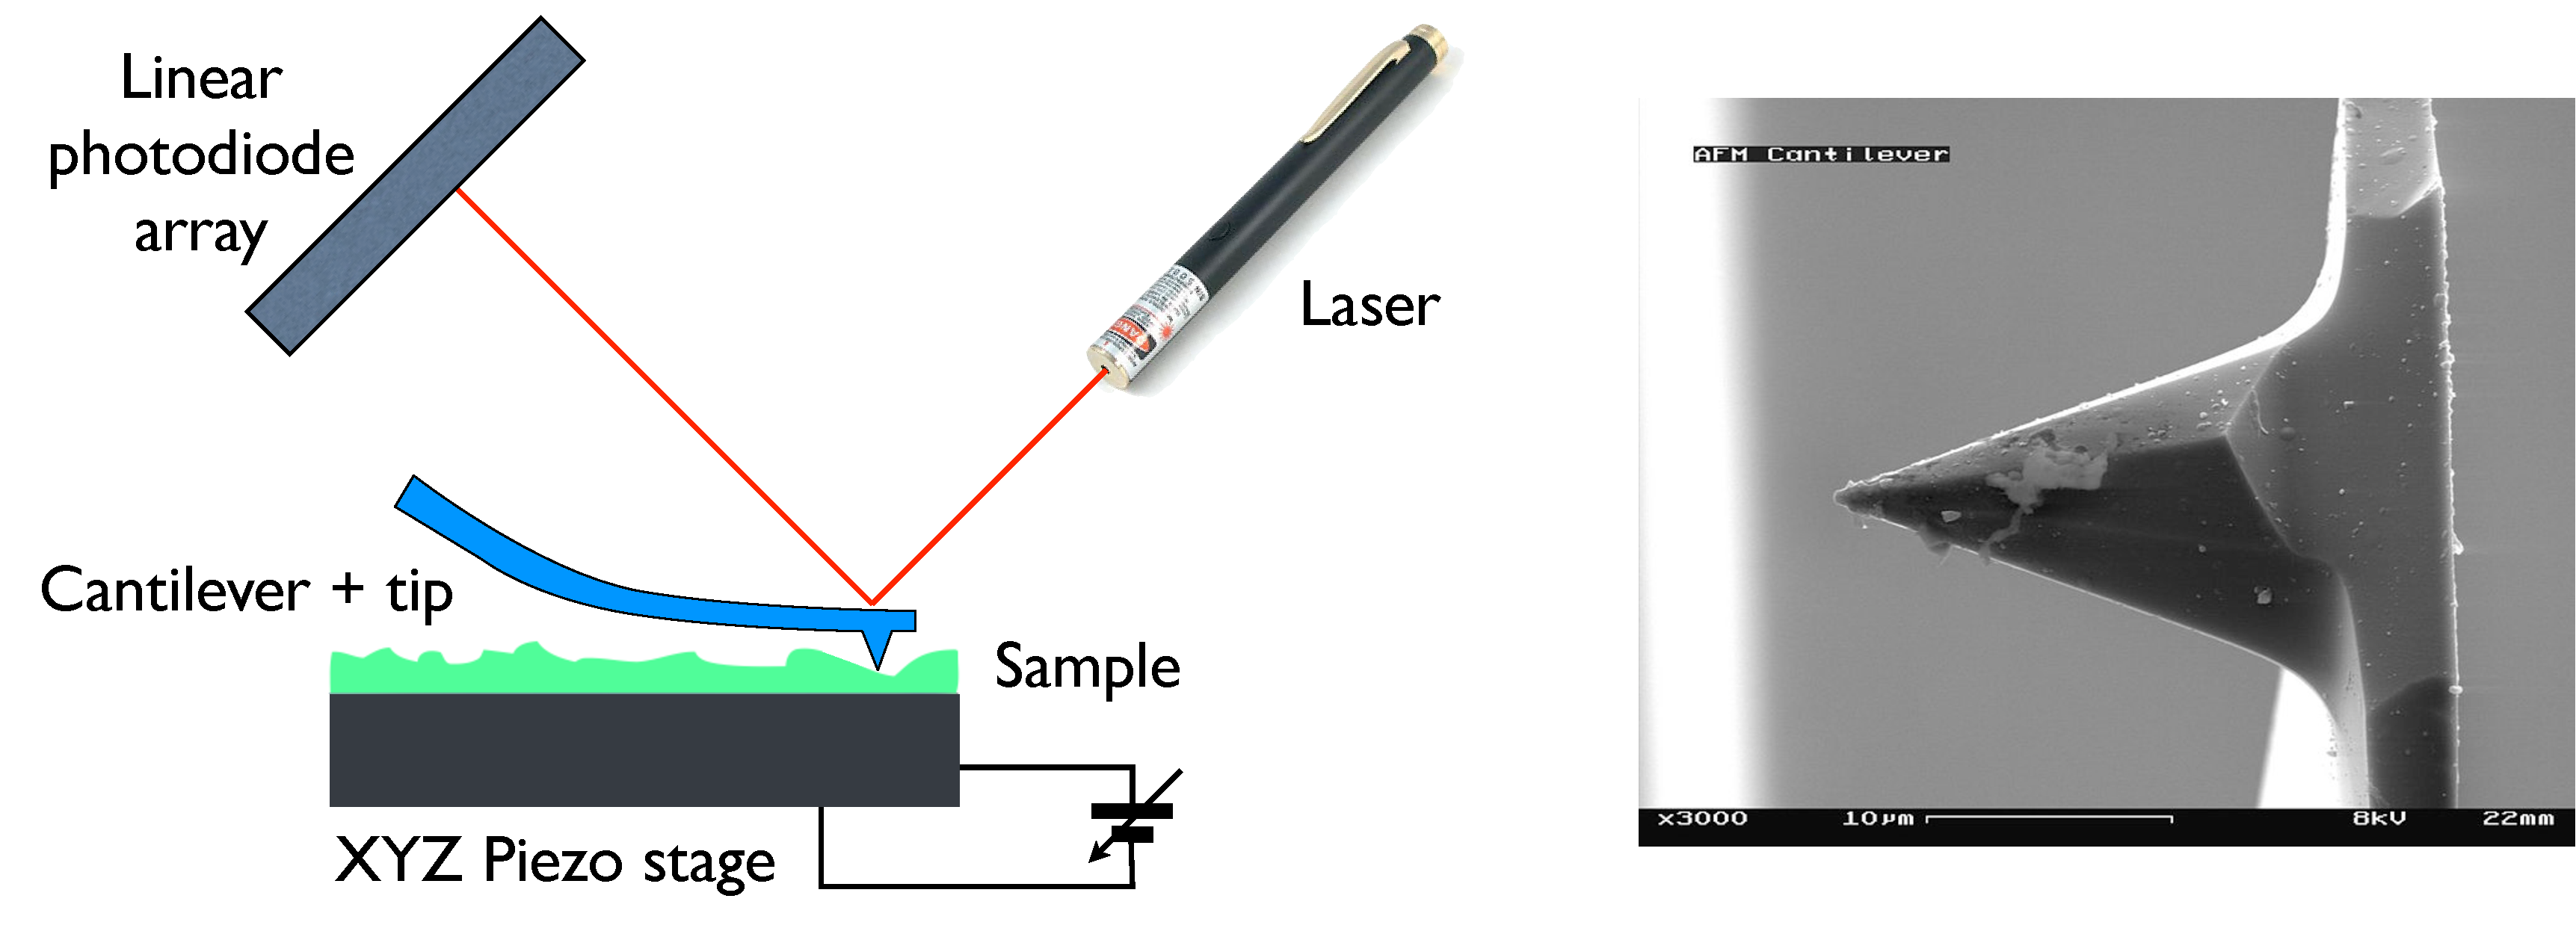
\includegraphics[width=1\textwidth]{Chapter5/5a_exampleAFM/afmSchematic.pdf} 
   \caption{Schematic diagram of an Atomic Force Microscope (AFM), and a Scanning Electron Microscope image of the tip, showing a radius of approximately 10 nm.}
   % TODO: cite the image from wikipedia. http://commons.wikimedia.org/wiki/File:AFM_(used)_cantilever_in_Scanning_Electron_Microscope,_magnification_3000x.JPG
   \label{afm}
\end{figure}

One limitation of AFM techniques is that it is easy to produce a two-dimensional map of the relative surface profile in arbitrary units, but difficult to accurately determine the absolute height.  In order to measure blaze angles of gratings, we need to measure the height difference from the bottom to the top of the grooves in absolute units, which requires calibration of the AFM using a height standard.  (Usually this is a gold mesh with an accurately-known wire size.)

After receiving the gratings from the manufacturer, we first imaged them using the AFM at the University of Saskatchewan Structural Sciences Centre (SSSC).  However, we were not able to calibrate the $z$-axis for these measurements, so with the assistance of Dr. Eric Gullikson, we requested a complete set of measurements using the AFM at the Center for X-Ray Optics at the Lawrence Berkeley National Laboratory.

An example of an AFM scan is given in Figure \ref{5a}, where we show both the two-dimensional image (top) and a cross-section of heights perpendicular to the grooves (bottom), which reveals the groove profile.  Although the grooves should be ideally uniform along their entire length, most of the AFM scans show profile variation across even one image (a distance of just a few micrometers).  To determine the average profile shape and average blaze angle, we integrated the two-dimensional image across the groove direction.  Since a single AFM scan only spans a few micrometers of the grating, we also need to be careful in extrapolating the results to the entire grating; therefore, we conducted multiple scans at the centre and the corners of the grating.

Figure \ref{5a} gives an example of the AFM output, for the LEG grating.  We present  groove profiles for all the gratings starting in Section \ref{gratingResults}, alongside a discussion of their effective diffraction performance.

\begin{figure}[htbp] %  figure placement: here, top, bottom, or page
   \centering
   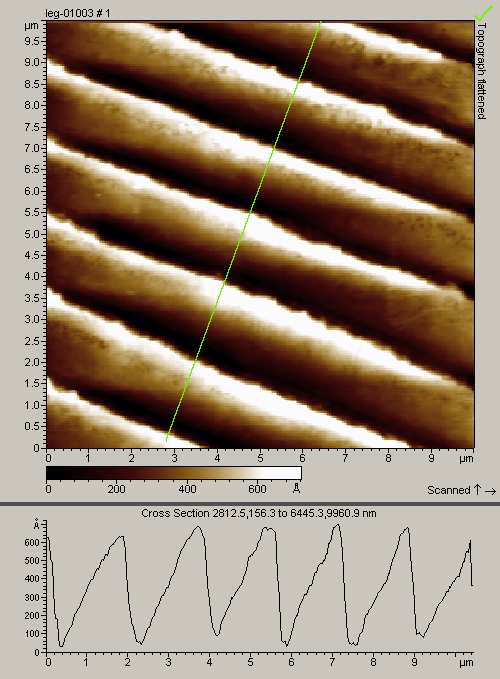
\includegraphics[scale=0.25]{Chapter5/5a_exampleAFM/afm_LEG_xsect1.png} 
   \caption{The Low Energy Grating has a smooth regular profile, shown in this example image measured using an Atomic Force Microscope (AFM).}
   \label{5a}
\end{figure}

\section{Diffractometer measurements of actual grating efficiency}
To measure the actual grating efficiency, we used the reflectometer on the Calibration and Standards Beamline (6.3.2) at the Advanced Light Source.  This beamline was designed specifically for testing the reflectivity of soft x-ray optical components like mirrors, thin films, multilayer coatings, and gratings.  It consists of a bending magnet source, a VLS-PGM monochromator with a resolving power of 7000 (Figure \ref{5b-a}), a higher-order suppressor, and a two-circle reflectometer (Figure \ref{5b}).  The beamline optics can focus the monochromator light to a small spot on the sample, or focus at infinite to generate parallel light \cite{Und96}.

\begin{figure}[htbp] %  figure placement: here, top, bottom, or page
   \centering
   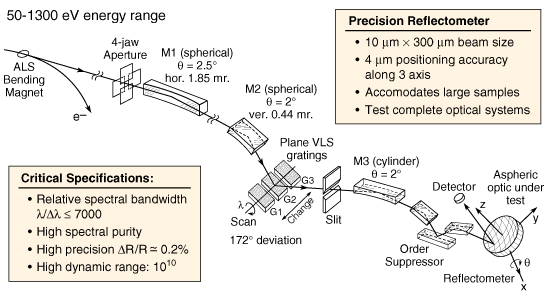
\includegraphics[scale=0.8]{Chapter5/5b_diffractometer/beamlineSchematic2.png} 
   \caption[The Calibration and Standards Beamline (6.3.2) at the Advanced Light Source consists of a bending magnet source, a VLS-PGM monochromator with three selectable gratings, a higher-order suppressor, and a two-circle reflectometer.]{The Calibration and Standards Beamline (6.3.2) at the Advanced Light Source consists of a bending magnet source, a VLS-PGM monochromator with three selectable gratings, a higher-order suppressor, and a two-circle reflectometer shown in more detail in Figure \ref{5b}.  The curvature of refocussing mirror M3 can be adjusted to image the exit slit onto the sample, or to focus the light at infinite.  Reprinted from Reference \cite{bl632}.}
   \label{5b-a}
\end{figure}

\subsection{Beamline 6.3.2 reflectometer}

\begin{figure}[htbp] %  figure placement: here, top, bottom, or page
   \centering
   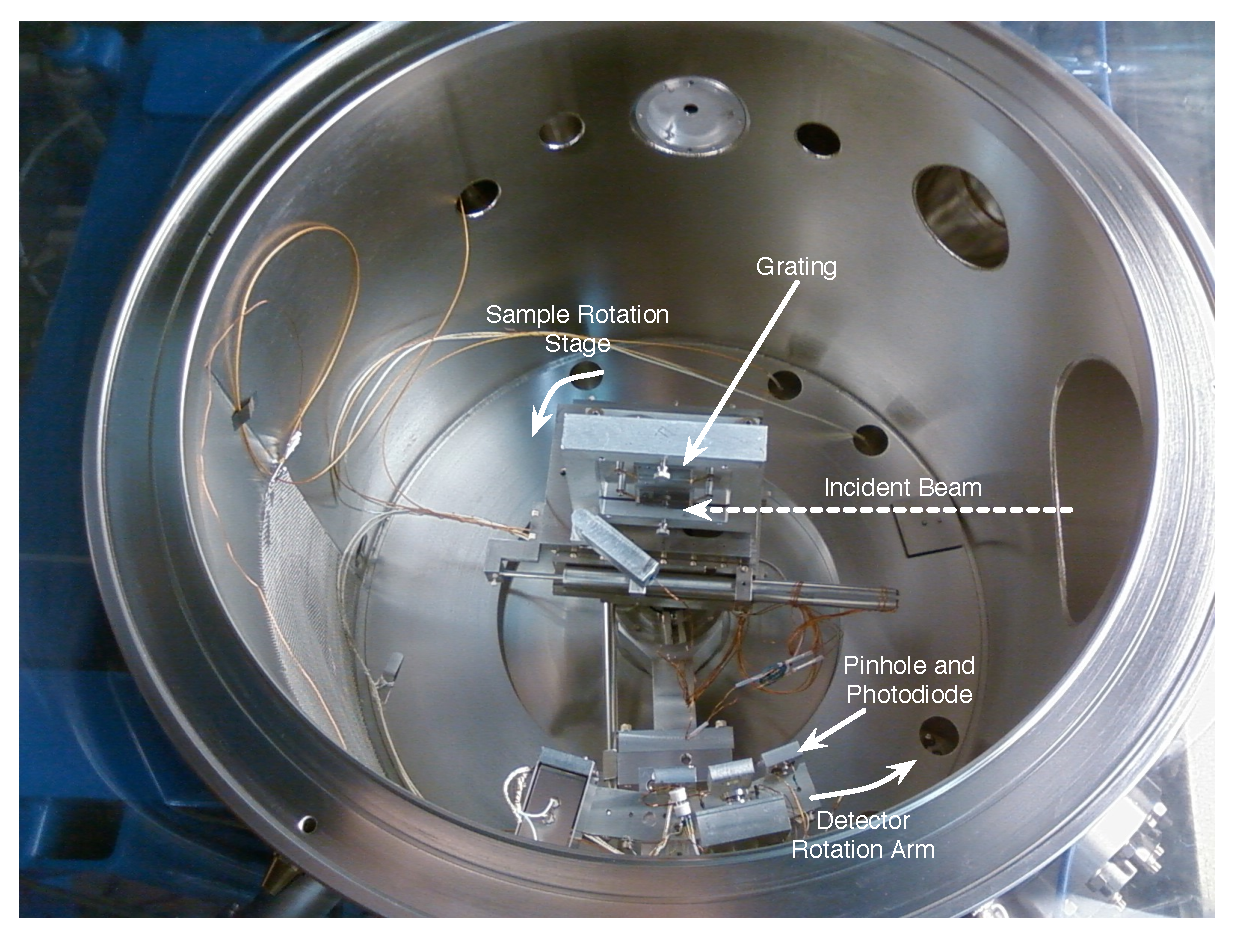
\includegraphics[scale=0.8]{Chapter5/5b_diffractometer/diffractometerLabelled2.pdf} 
   \caption[The reflectometer on Beamline 6.3.2 at the Advanced Light Source allows for independently setting the angle of the gratings in the beam, and setting the angle of a pinhole photodiode detector.]{The reflectometer on Beamline 6.3.2 at the Advanced Light Source allows for independently setting the angle of the gratings in the beam, and setting the angle of a pinhole photodiode detector.  Upstream, filters in the beamline are used to remove contamination from the higher-order light of the monochromator. }
   \label{5b}
\end{figure}

The purpose of the reflectometer endstation (Figure \ref{5b}) is to measure the intensity of light reflected off a sample -- in our case, a grating -- as a function of both incidence and reflection angle.  We used it to determine grating efficiency by positioning the grating at the intended incidence angle relative to the incoming beam,  measuring the intensity at the angle of the outgoing order, and comparing this to the initial beam intensity.  Upstream, the monochromator and order suppressor were used to produce the monochromatic incident beam and set its energy for each datapoint.

\begin{figure}[htbp] %  figure placement: here, top, bottom, or page
   \centering
   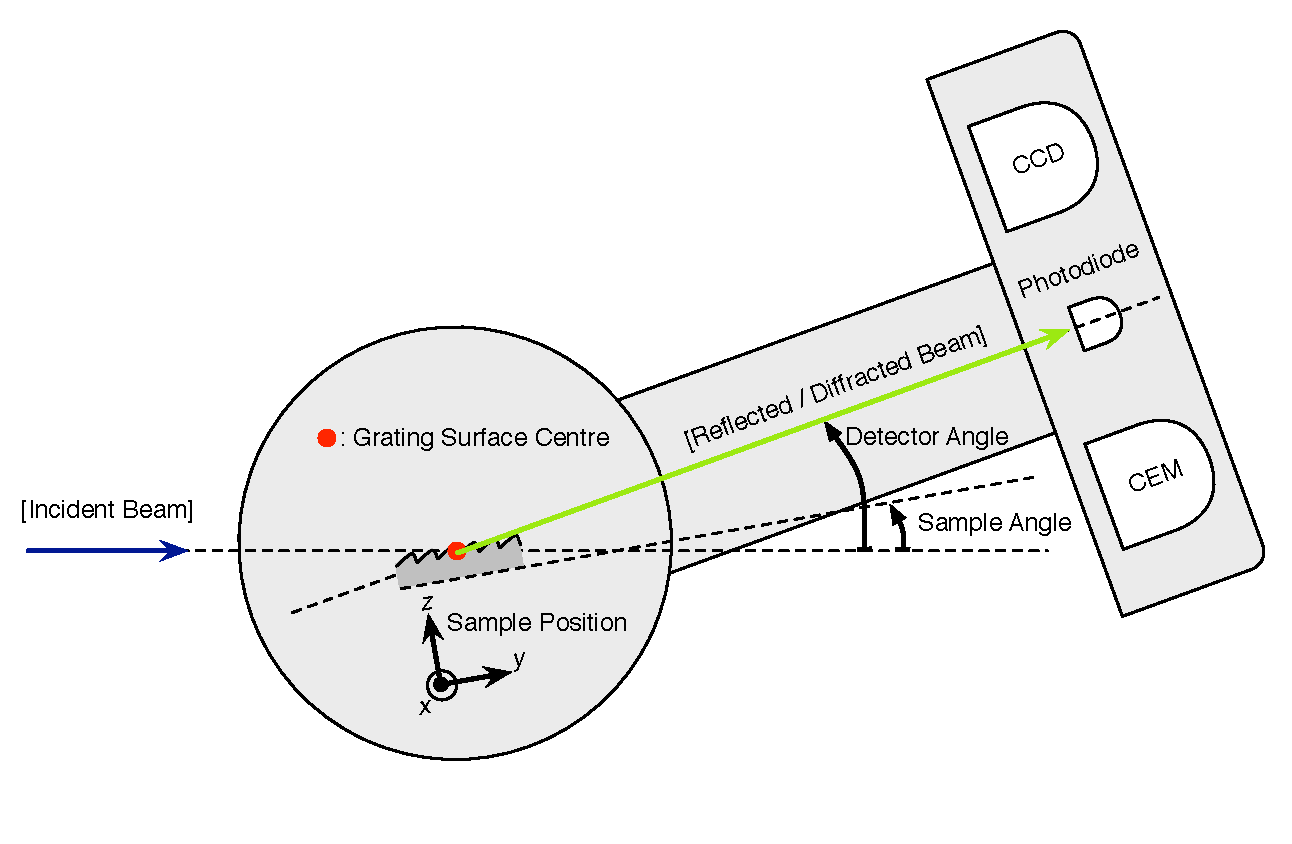
\includegraphics[scale=0.8]{Chapter5/5b_diffractometer/reflectometerCoordinates.pdf} 
   \caption[Reflectometer coordinates: the sample angle is measured up from grazing incidence, and the detector angle is measured up from grazing incidence.]{In the coordinate convention for the reflectometer, the sample angle is measured up from grazing incidence, and the detector angle is measured up from grazing incidence.  The sample position stage ($x$, $y$, $z$) is mounted to the sample angle stage, so that the centre of rotation is always at the height of the beam.}
   \label{reflectometerCoordinates}
\end{figure}

Inside the reflectometer mechanics, a ``two-circle goniometer'' provided independent control over the angle of the sample and the angle of the detector arm, as well as providing precise (4 um) positioning to align the sample in $x$, $y$, and $z$.  (Figure \ref{reflectometerCoordinates} shows the coordinate system convention, with angles measured from grazing incidence or inline with the beam; the ``0 degree'' sample position would place the grating at perfect grazing incidence, while the ``0 degree'' position for the detector would capture the incoming beam when unobstructed.)  The sample holder could accommodate samples up to 200 mm in diameter, which allowed us to mount two of our gratings side-by-side at once.  The detector arm contained a Hamamatsu gallium arsenide photodiode, a channel electron multiplier (CEM, or ``channeltron''), and a CCD camera. For all of our grating measurements, we used the photodiode covered by a 2 mm pinhole.

\subsection{Diffraction experiment procedure}
\label{procedure}
Diffraction efficiency measurements are easily susceptible to a variety of systematic and unintentional errors.  The following sections describe in detail the procedure we used for measuring the grating efficiency, and how we dealt with sources of error.
\subsubsection{Grating Alignment}
To achieve correct incidence angles and accurate detection angles, the grating had to be aligned correctly.  In the $z$-direction (Figure \ref{reflectometerCoordinates}), the centre of the grating surface had to coincide with the centre of sample rotation, which was also aligned to the height of the beam.  In the $x$-direction (parallel to the grating grooves), the beam had to land on the centre of the grating; otherwise the curvature of the grating would introduce a slope in the saggital direction, and we would end up with conical mounting.
	\begin{enumerate}
	\item To crudely align the grating in the $z$-direction, the grating angle was set to zero degrees, and the CCD camera was placed at a detection angle of 0 degrees.  With the sample moved fully down out of the way in $z$, this allowed the beam to shine past the grating directly onto the centre of the CCD, confirming the alignment of the beam angle. 
	\item The grating was then moved upward in $z$ until it just started blocking the beam from reaching the CCD detector, indicating that the surface was now at (or just above) beam height.
	\item With the grating blocking the CCD detector in this position, it was translated in $x$ until light returned, indicating that the beam had fallen off the side edge of the grating.  This was repeated in the $(-x)$-direction, providing us with the position of the opposite side; the grating was then positioned midway between these two positions, achieving alignment in $x$.
	\item To accurately complete the alignment in $z$, the grating was angled at two degrees, and the photodiode detector was positioned to collect reflected (0th order) light at four degrees.  As long as the beam was incident on the grating, this would register a signal on the detector.  The grating was then translated upward in $z$ until the signal disappeared, indicating that the beam had fallen off the bottom edge of the grating. This $z$-position was recorded as the bottom grating edge.
	\item The grating was then lowered in $z$ until the signal disappeared again, indicating that the beam had fallen off the top edge of the grating.  This $z$-position was recorded as the top grating edge, and then the grating was moved to the average of the two recorded $z$-positions; this process ensured that the beam was now incident on the exact centre of the grating.
	\end{enumerate}
	
\subsubsection{Scanning modes}
All of the efficiency plots we calculated in Chapter 6 to predict the REIXS gratings' performance show efficiency as a function of photon energy.  We wanted to show our real-world measurements in the same format, which required us to scan the monochromator energy while measuring the intensity of the desired order with the photodiode.  Therefore, the detector angle had to change as we changed the monochromator energy, according to the outgoing angle specified by the grating equation \eq{gratingEquation}.  

If we had known the groove density with high accuracy, we could have calculated the correct diffraction angle and positioned the detector simultaneously while scanning the monochromator energy.  However, for brand new gratings, it would be unlikely for the groove density to end up exactly as requested from the manufacturer; in this case we would actually need to conduct a two-dimensional scan: for every photon energy datapoint, we would need to conduct an angular scan of the photodiode to find the diffraction peaks.\footnote{After completing this scan, we could use the angular position of the diffraction peaks to calculate the actual groove density, but only within a precision determined by the angular extent of the 2mm photodiode pinhole.}

For four of the gratings, we did have an accurate groove density, obtained from Power Spectral Density (PSD) measurements taken by the metrology lab at the Canadian Light Source.  However, for two of the gratings, the exact groove density was unknown, so we had to use the two-dimensional scan method.  Mechanically, this is the simplest way to operate the reflectometer, and an example of the results are shown in Figure \ref{5c}.  The procedure was as follows:

	\begin{enumerate}
	\item The monochromator was set to the desired photon energy, and the corresponding filters were selected in the higher-order absorber.
	\item The grating was positioned at its specified incidence angle relative to the beam, as it would be during operation of the spectrometer.
	\item The photodiode was scanned, recording intensity as a function of outgoing angle.
	\item The grating was moved out of the way of the beam, and the photodiode was placed at zero degrees to measure the direct beam intensity; this intensity value was used to normalize the data as described later in this section. 
	\item The results (Figure \ref{5c}) show the intensity of reflected light as a fraction of the incident beam intensity, as a function of detector angle.  The 0th order, 1st order, and 2nd order peaks are clearly seen; we can quickly check that the 0th order peaks show no wavelength dependency and occur at twice the incidence angle.  The grating efficiency in the $n$th order is taken from the height at the centre of the $n$th diffraction peak.
	\end{enumerate}

This time-consuming procedure had to be repeated for every photon energy datapoint that we wanted to test.  For the gratings where the groove density was known accurately, we used a more expedient method, which required synchronized scanning of the detector angle and monochromator energy:

	\begin{enumerate}
	\item The higher-order suppressor was configured for the energy range of the scan. (This limited each individual scan to the valid energy range of a single higher-order filter; see Section \ref{higherOrderContamination})
	\item The control software was configured to move the detector angle in tandem with the monochromator energy to stay on top of the diffraction peak, using the grating equation and the specified groove density and order.
	\item The monochromator energy and the detector angle were scanned together, recording the intensity of the diffracted order at each datapoint.
	\item The grating was then moved out of the way of the beam, and the detector angle was set to zero degrees to measure the direct beam.  The monochromator energy scan was repeated to measure the incident intensity as a function of energy, to use for normalization (see `Normalization', below).
	\item An example of the normalized results is shown in Figure \ref{5d}. They directly show the intensity of diffracted light in the specified order as a fraction of the incident beam intensity, as a function of energy.  With this method, it is easier to measure a finely-spaced set of datapoints along the energy axis, to compare with our efficiency prediction plots in Chapter 6.
	\end{enumerate}

\begin{figure}[htbp] %  figure placement: here, top, bottom, or page
   \centering
   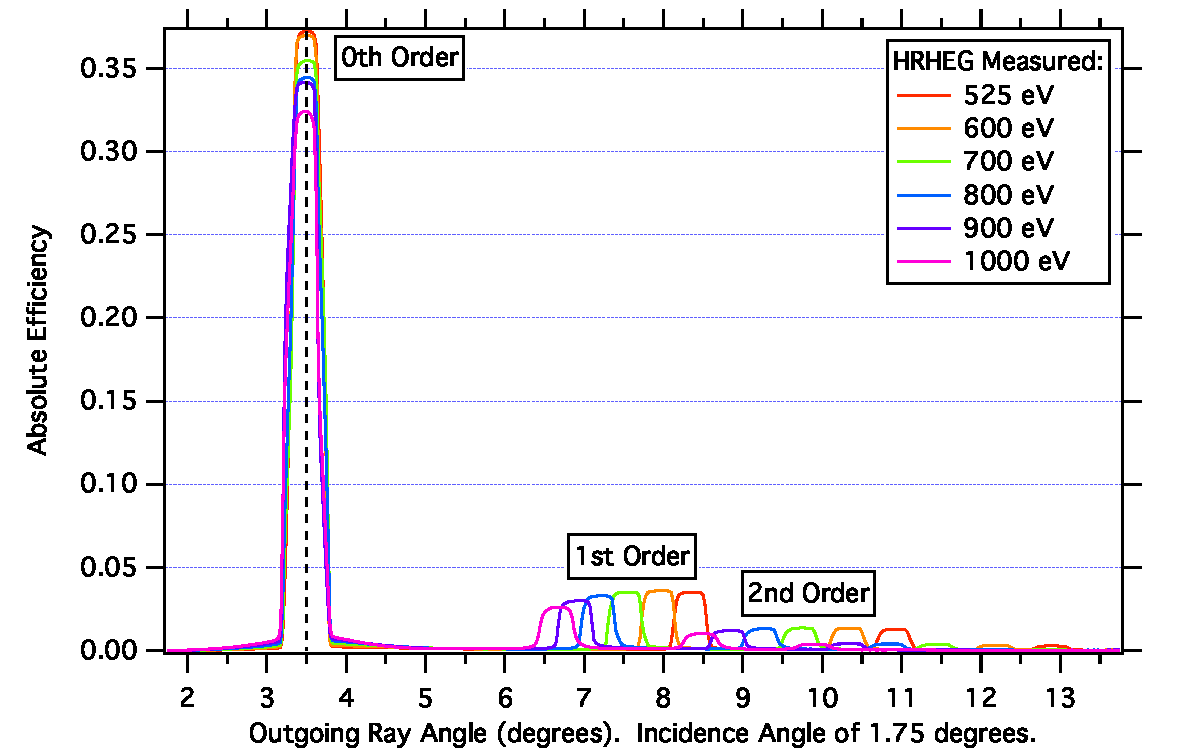
\includegraphics[scale=0.8]{Chapter5/5c_angleScan/5c_solidColors.pdf} 
   \caption[The simplest diffractometer experiment scans the detector angle while illuminating the grating with a constant photon energy.]{The simplest diffractometer experiment scans the detector angle while illuminating the grating with a constant photon energy.  The diffraction orders are visible as peaks along the outgoing angle axis (measured up from the incident beam direction at 0$\deg$).  The 0th order (reflection) peak is easily visible at 3.5$\deg$, or twice the incident angle (88.25$\deg$, or 1.75$\deg$ from grazing).  Grating: HRHEG.}
   \label{5c}
\end{figure}

\begin{figure}[htbp] %  figure placement: here, top, bottom, or page
   \centering
   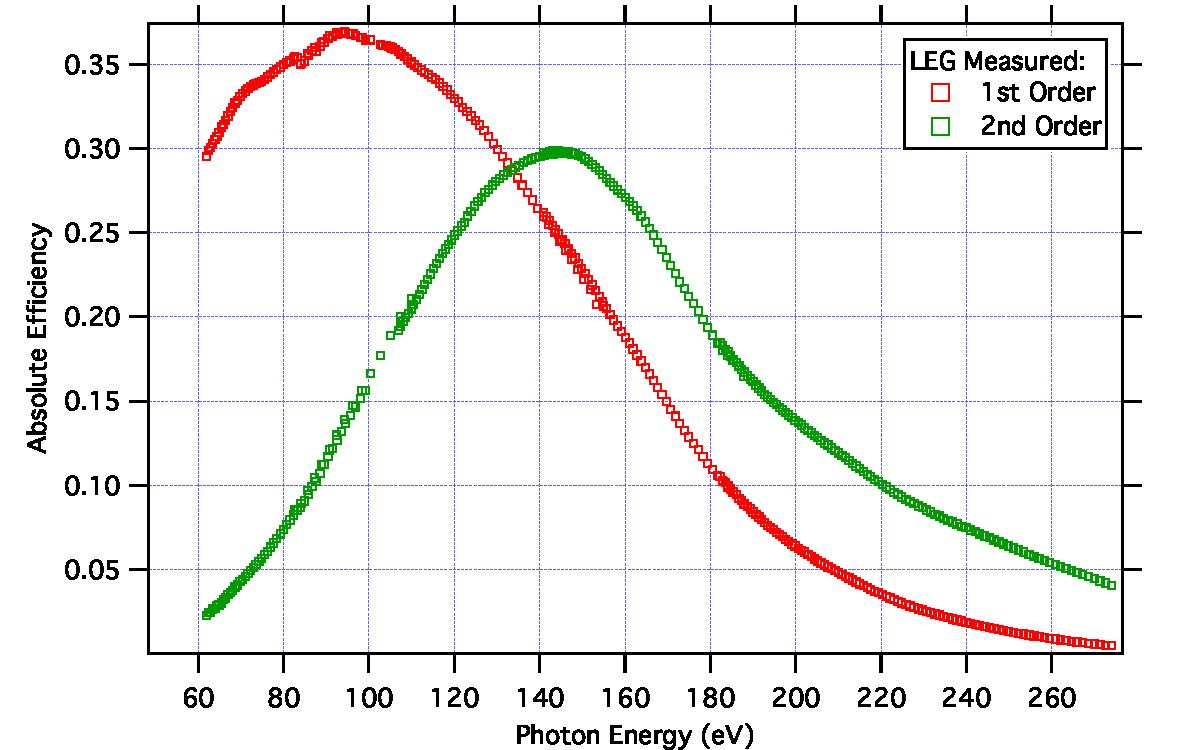
\includegraphics[scale=0.8]{Chapter5/5d_energyScan/5d_LEG.pdf} 
   \caption[When the groove density of a grating is accurately known, the detector angle can be moved in tandem with the monochromator energy to keep it on the diffraction peak as the incident photon energy is scanned.]{When the groove density of a grating is accurately known, the detector angle can be moved in tandem with the monochromator energy to keep it on the diffraction peak as the incident photon energy is scanned.  This allows faster, nearly continuous efficiency measurements as a function of photon energy.  (Grating: LEG)}
   \label{5d}
\end{figure}

\subsubsection{Wavelength calibration}
The monochromator on Beamline 6.3.2 is slitless, therefore its absolute energy calibration is affected by the position of the beam in the ALS storage ring.  To calibrate the energy axis of our data, we scanned the monochromator through the absorption edges of the higher-order suppression filters, and compared the onset of the edges with the published values for the binding energies of these elements:
	\begin{enumerate}
	\item For every new energy range, monochromator grating change, or storage ring refill, the sample was moved out of the way and the photodiode was placed at 0 degrees to measure the direct beam.
	\item The monochromator was scanned upward in energy through the onset of the nearest absorption edge of a filter placed in the beam path.  (For example, prior to doing scans in the energy range from 82.6 to 112 eV, we installed the silicon filter and scanned across the Si $L3$ absorption edge, located at 99.42 eV.)  Essentially, this amounted to measuring a transmission x-ray absorption spectrum of the filter element.
	\item The wavelength shift of the onset of the absorption edge (in monochromator wavelength units) away from its theoretical position provided a correction offset that was applied to the wavelength axis for all scans in this range.\footnote{The monochromator control software used wavelength units rather than energy units, so we conducted all of our efficiency scans in wavelength units and converted later from nm to eV, using the photon energy relationship $E=hc/\lambda$.}
	\end{enumerate}
	
\subsubsection{Normalization}
\label{normalizationEff}
Chapter 3 defined grating efficiency as the ratio of the intensities of the $n$th order diffracted beam and the incident beam.  In our measurement procedure (above), we used the photodiode to record the intensity of the reflected beam $I_r$, and subsequently the intensity of the incident beam $I_i$.  The efficiency $e^{(r)}$ would then be
\begin{align}
e^{(r)} = \frac{I_r}{I_i}
\end{align}
Using the same detector to measure both the reflected and incident beam eliminates error due to differences in detector sensitivity.  However, because these measurements were not taken simultaneously, it is possible that the incident beam intensity would have changed in the interim; in fact, this would be virtually guaranteed due to decay of the storage ring current over time.  Because the light intensity of a bending magnet beamline is proportional to the storage ring current $J_{\mathrm{ring}}$, we can record the ring current at the time of each measurement, and use it to normalize the intensities:
\begin{align}
e^{(r)} = \frac{I_r / J_{\mathrm{ring},r}}{I_i / J_{\mathrm{ring},i}}
\end{align}

Finally, as we identify in the following section, the dominant source of error in low-light photodiode measurements is the \emph{dark current}: an intensity-independent signal from the photodiode that increases with temperature due to thermal generation of electron-hole pairs.  With the beam blocked, we measured the dark current $I_{\mathrm{dark}}$ for every gain setting of the photodiode, and subtracted this  contribution from all measurements to determine the true intensity ratio:
\begin{align}
e^{(r)} = \frac{(I_r - I_{\mathrm{dark}}) / J_{\mathrm{ring},r}}{(I_i - I_{\mathrm{dark}})/ J_{\mathrm{ring},i}}
\label{effNormalization}
\end{align}
We used Equation \eq{effNormalization} to normalize all of the efficiency results in Section \ref{gratingResults}.

\subsection{Sources of error}
\label{sourcesOfError}
In the previous description of our procedure, we briefly mentioned the ``higher-order suppressor'', the dark current, and the energy calibration.  In this section, we take a look at all of the sources of error which could affect the grating efficiency measurements.
\subsubsection{Higher-order contamination}
\label{higherOrderContamination}
A bending magnet source like the one on Beamline 6.3.2 produces light of all wavelengths, from infrared to hard x-rays; it is the responsibility of the monochromator to extract a single wavelength from this broadband input.  The problem with grating monochromators, however, is that the grating equation cannot distinguish between equivalent products of $n$ and $\lambda$: light with a wavelength of $x$ nanometers diffracted in 1st order will leave at the same angle as $x/2$-nanometer light diffracted in 2nd order.\footnote{In terms of energy, photons with an energy of $y$ eV will diffract in 1st order to the same angle as $2y$-eV photons in 2nd order.}  When both wavelengths are present in the monochromator input, this creates what is known as ``higher-order contamination'' in the output.  Because the monochromator gratings are likely more efficient in 1st order than any other, the intensity of $x/2$ and $x/3$-nanometer light will be comparatively lower than the desired wavelength, but it will still contaminate the mono output.  If this higher-order light were to arrive at the grating under test, it would be diffracted again, introducing additional erroneous peaks into the detector angle scan.  (Depending on the ratio of the monochromator and test-grating groove densities, these erroneous peaks could either overlap or fall beside the ``true'' diffraction peaks.)  Therefore, reflectometry experiments require a method to eliminate this higher-order light before it reaches the sample.

Beamline 6.3.2 has two techniques for higher-order suppression.  The first is a variable-incidence mirror with multiple sets of coating stripes.  This design exploits the change in reflectivity as a function of incidence angle and energy that we saw (for example) in Figure \ref{reflectionVsAngle}.  Depending on the desired wavelength, the mirror coating and grazing angle are chosen to provide high reflectivity at the desired wavelength, but significantly lower reflectivity at fractionally shorter wavelengths.

The second technique is a filter wheel containing a set of transmission filters from various elements which may be inserted into the beam path prior to the endstation.  The filters are between 300 nm and 1 um thick, and are designed to remove 50\% or more of the light at energies above the filter's absorption edge.

Table \ref{filterTable} shows the mirror coating, mirror angle, and filter element that we used for higher-order suppression.  The energy ranges of each mirror/filter combination (shown in the left column) restricted the maximum extent of each efficiency scan; for the efficiency results shown in Section \ref{gratingResults}, we have combined multiple scans together.

\begin{table}[htbp]
   \centering
   \topcaption[For higher-order suppression, Beamline 6.3.2 has a variable-incidence mirror and a set of transmission filter elements.  The mirror coating, mirror angle, and filter need to be selected based on the energy range of the scan.]{For higher-order suppression, Beamline 6.3.2 has a variable-incidence mirror and a set of transmission filter elements.  The mirror coating, mirror angle, and filter need to be selected based on the energy range of the scan.  (Mirror angles are measured from grazing incidence.)}
   \begin{tabular}{@{} c l c l @{}} % Column formatting, @{} suppresses leading/trailing space
\toprule
Energy Range	(eV) &	Mirror	&	Mirror Angle ($\deg$)	&	Filter	\\
\midrule
62 - 99	&	\multirow{4}{*}{Carbon}	&	\multirow{2}{*}{10}	&	Silicon	\\
83 - 112	&			&			&	Beryllium	\\
\cmidrule(l){3-4}
103 - 155	&			&	8	&	\multirow{2}{*}{Boron}	\\
141 - 188	&			&	6.2	&			\\
\midrule
182 - 276	&	\multirow{2}{*}{Nickel}	&	\multirow{2}{*}{8}	&	Carbon	\\
275 - 454	&			&			&	[None]	\\
\midrule
441 - 546	&	\multirow{4}{*}{[None]}	&		&	Chromium	\\
544 - 775	&			&		&	Cobalt	\\
751 - 932	&			&		&	Copper	\\
898 -  1305&			&		&	Magnesium	\\
\bottomrule
   \end{tabular}
   \label{filterTable}
\end{table}

\subsubsection{Monochromator energy calibration}
The monochromator is approximately calibrated; entering a desired wavelength into the control software -- for example, 2.73 nm -- will align the mono grating to diffract light of approximately 2.73 nm out through the exit slit.  However, the calibration is not perfect, and it is also affected by shifts in the ALS electron beam orbit position.  Therefore, it is important to obtain an absolute wavelength calibration whenever moving to a substantially different wavelength range, changing monochromator gratings, or resuming scans after a storage ring refill.

As described in the procedure, we calibrated the wavelength axis of our efficiency scans (eventually, the energy axis) by conducting transmission absorption spectroscopy on the filter elements in Table \ref{filterTable}.  The difference between the monochromator's apparent wavelength at the halfway height of the absorption edge, and the wavelength corresponding to the published binding energies for those elements, was used to generate a wavelength offset for nearby scans.  (The monochromator's calibration might also suffer from errors which require linear and quadratic scaling corrections, but we assumed that a simple offset would be sufficient over the short length of these scans.)

\subsubsection{Photodiode dark current}
Photodiodes can be operated in a forward-biased (\emph{photovoltaic}) mode, or in a reverse-biased (\emph{photoconductive}) mode.  When used as sensitive detectors of light intensity, the photoconductive mode is almost always used, because it offers faster response times and a linear response to light intensity over many orders of magnitude.  In this mode, a reverse bias is applied and -- in the absence of light -- only a small \emph{dark current} flows through the diode, due to the thermal generation of electron-hole pairs in the $p-n$ junction.  When light strikes the $p-n$ junction, incident photons create electron-hole pairs which are swept across the junction by the reverse bias, and create an intensity-dependent \emph{photocurrent}.  The total current through the photodiode is measured by a sensitive current amplifier.

The dark current depends on temperature, and slightly on the magnitude of the reverse bias voltage.  (In our instrumentation, the reverse bias was affected by the gain setting of the current amplifier.)  To account for this, we measured the dark current at every gain setting with the beam turned off, and then subtracted this in the normalization equation \eq{effNormalization}.  The dark current measurements were conducted after the diode had been operating under reverse bias for some time (and hopefully had reached operating temperature).  Since the dark current increases with temperature, it is possible that exposure to extreme intensity would heat the detector and change the dark current contribution; however, this effect should be negligible for the low intensities observed in our experiment.

\subsubsection{Saggital tilt of the grating}
The reflectometer mechanics enable the intended rotation of the sample (grating) around the $x$-axis in FIgure \ref{reflectometerCoordinates}.  If the grating surface were tilted away from normal incidence around the $y$-axis -- either due to an offset in the grating mount, or due to the curvature of the grating combined with incorrect alignment in the $x$-direction -- light would be reflected out of the $y-z$ plane.  This would create the ``conical mount'' situation we assumed we could avoid modelling in Chapter 3, and would also cause the diffracted beam to partially or completely miss the 2 mm pinhole of the photodiode detector.  Both of these effects would reduce the observed intensity from what we would expect.

The zero-order alignment test we described in the procedure confirmed that with the grating positioned at 2 degrees, a substantial current was observed on the photodiode at 4 degrees, indicating that a substantial amount of light was staying within the plane of incidence.  However, we cannot confirm that the alignment was flawless, and it is possible that the measured efficiencies are lower than they would be under perfect alignment.

\subsubsection{Limited beam spot size}
The Beamline 6.3.2 optics focus the beam to a spot size of 0.010 mm x 0.3 mm on the grating.  
%(TODO check if we were focussed at grating or infinite.)
Because the grating needs to be aligned on the centre of rotation, there can only be one position for the beam on the grating, and so we could only test the efficiency at this point.  If there is variation in the groove profile across the grating, the illuminated part of the grating may not actually be representative of the average efficiency.  

It is impossible to overcome this limitation; even if it were possible to fully illuminate the grating, the grating curvature would not be correct to focus the diffracted beam to the same size on the detector as the incident beam would be.  Therefore, a small beam size is a necessary compromise to minimize the focussing effect of the grating.

%\subsubsection{Energy dispersion across detector pinhole (finite size of pinhole + finite resolution dE)}
%TODO need to discuss with Eric Gullikson
%\subsubsection{Focussing / Defocussing}
%TODO TODO Important (need to discuss with Eric Gullikson?)

\section{Real-world grating effects}
\label{realWorldEffects}
The comparisons between the predicted and measured efficiencies for each grating are discussed in Section \ref{gratingResults}, and impatient readers might have already beat us there.  However, before looking at the results, it might be useful to consider some of the factors that could cause a discrepancy between the two.  If there are differences between the predicted and measured efficiency, this would imply one -- or more -- of three distinct possibilities:
\begin{enumerate}
\item That the measurement procedure, due to experimental error, did not measure the actual grating efficiency.
\item That the theory and calculation method do not correctly describe the gratings they attempted to model,\\
or,
\item That the real-world gratings, as produced, are different from the ones we modelled.
\end{enumerate}
We dealt with the first possibility in the previous section on sources of error.  Before accepting the second possibility, we take a look at some of the ways manufactured gratings differ from ideal ones.

\subsection{Stray radiant energy}
For a perfectly periodic surface, the Rayleigh expansion in Chapter 3 showed that all of the light propagating away from a grating leaves as plane waves in discrete orders. Regardless of the groove shape, no light leaves except at the angles given by the grating equation \eq{gratingEquation}.  In real-world gratings, deviations from perfect periodicity lead to \emph{stray radiant energy} (SRE), which is a general term for all radiation that leaves at other angles \cite{RicTN9}. From conservation of energy, the more SRE that exists, the less energy there is in the desired orders, and the lower the grating efficiency.  SRE also affects the resolution of a grating instrument, by increasing the background noise level and contaminating the outgoing angles with light of the wrong wavelength.

Stray radiant energy can be caused by micro-roughness of the grating surface, variation in the height or spacing from groove to groove, and other imperfections such as dust and scratches.
\subsubsection{Surface roughness}
The grating model in Chapter 3 assumed a perfectly smooth surface, given by the periodic profile $y_p=g(x)$ in Figure \ref{2a}.  Unfortunately, both ruling and coating processes invariably leave a certain amount of micro-roughness, shown exaggerated in Figure \ref{5e}.  When the surface is rough on the scale of the incident wavelength, it causes diffuse scattering, which is analogous to the diffuse (or non-specular) reflection that would occur off any rough surface.  Because this phenomenon affects the entire  area of the grating, diffuse scattering from surface roughness is typically responsible for most of the reduction in real-world grating efficiency (compared to theoretical calculations).

\begin{figure}[htbp] %  figure placement: here, top, bottom, or page
   \centering
   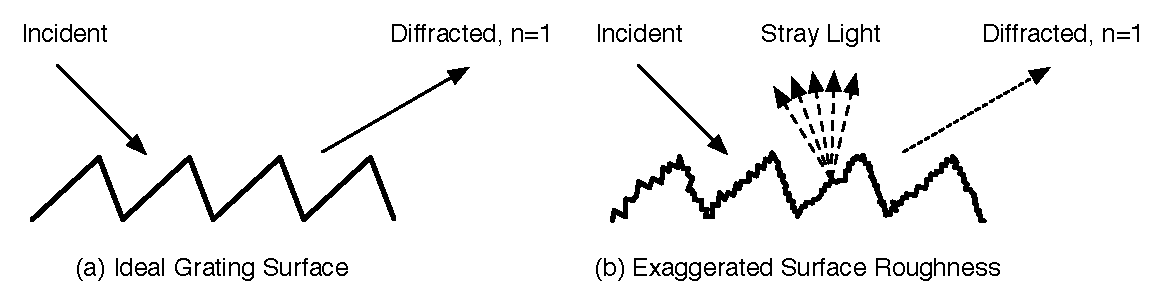
\includegraphics[scale=0.8]{Chapter5/5e_surfaceRoughness/5e.pdf} 
   \caption{Roughness of the grating surface scatters stray light outside the diffraction orders. Typically, surface roughness is responsible for most of the reduction in real-world grating efficiency, compared to theoretical calculations.}
   \label{5e}
\end{figure}
 
Although it might not be clear from Figure \ref{5e} -- which is two-dimensional -- diffuse scattering need not be constrained to the plane of incidence. The roughness creates slope variation in both $x$ and $z$, so scattered light could end up anywhere in the hemisphere above the grating.  However, in-plane scattering is stronger than out-of-plane scattering by a factor of $1/\cos\theta$ (where $\theta$ is the incidence angle from normal). Therefore, at grazing incidence, the in-plane scattering is dominant \cite{Sch02}.

To correct the predicted grating efficiencies for scattering, we need to understand two things:
\begin{enumerate}
\item The amount of energy lost to scattering, as a function of roughness, wavelength, incidence angle, and diffraction order.
\item The angular distribution of the scattered intensity. Does it affect all diffraction orders the same way?
\end{enumerate}

Given the randomness of the surface structure, we need statistical methods to answer these questions.  Statistically, the surface roughness is characterized by $\sigma$, the root mean square (RMS) variation in height from the nominal plane, and by the power spectral density (PSD) function, which describes how the height variation is distributed in frequency.
%\footnote{Because the surface height is ``stationary random process'' -- i.e.: the mean and variance do not change over position -- the PSD is the Fourier transform of the autocorrelation function of the height $h(x)$.}

Even for the simpler (non-grating) case of roughness on flat surfaces, a substantial amount of research has only succeeded in producing a murky swamp of approximate models.  In Reference \cite{Elf04}, Elfouhaily and Guerin categorized 260 references -- 177 since 1980 -- into 30 different methods, before concluding that ``there does not seem to be a universal method that is to be preferred systematically. All methods present a compromise between versatility, simplicity, numerical efficiency, accuracy and robustness, with a different weighting in these various fields. [...] No approximate model has fulfilled all listed criteria.''

Even though they only deal with nominally flat surfaces, all of these methods are based on the assumption that a random rough surface can be decomposed into a superposition of sinusoidal gratings\footnote{Obviously, in our case, of much higher groove density than the actual gratings!}, and that scattering can be explained as a diffraction effect from the phase changes created by the ``microtopography'' of the surface \cite{Rag07}.  There are two fundamental approaches: the Rayleigh-Rice theory \cite{Ray07,Ric51}, which is a perturbation approximation for solving the electromagnetic vector wave equation near periodic interfaces, and the Beckmann-Kirchhoff theory, which uses a scalar wave equation and applies the Kirchhoff diffraction formula \cite[Chapters 4 and 5]{Bec87}.  Both contain approximations; the Rayleigh-Rice methods are only applicable to ``smooth'' surfaces, where the perturbation from a flat surface is small -- i.e., where the RMS roughness is small compared to the wavelength ($\sigma \ll \lambda$).  The Beckmann-Kirchhoff methods are appropriate for ``rougher'' surfaces up to $(\sigma \cos \theta \leq \lambda)$, but they contain a small-angle approximation that restricts them to near-normal incidence and scattering angles \cite{Rag07}.  (In the extreme case where the roughness is much larger than the wavelength, it becomes more appropriate to handle it using a geometric optics approach, rather than a diffraction approach.  In this situation, we can imagine a surface made up of many ``microfacets'' all reflecting light at different angles; the BESSY raytracing software suite actually uses this approach to model roughness by randomly varying the direction of a mirror's normal vector (slightly) for each reflecting ray, according to the statistical description of the surface \cite{Sch}.)

Since grating theories are already being used to describe diffuse scattering from rough \emph{flat} surfaces, applying these methods to \emph{actual} gratings is even more difficult; this amounts to creating a superposition of (very high density) gratings, \emph{on the surface of another grating}.
 
 It would be theoretically difficult to analyze ``gratings structured on top of gratings'', so instead, we apply some of the results for rough mirrors to come up with an approximate correction for our grating efficiencies.  Many texts and computer programs use a simple expression called the ``Beckmann factor''
\begin{align}
\label{beckmannFactor}
R' &= R \exp\left(  - \left(\frac{4\pi\sigma \,  \cos \theta}{\lambda}\right)^2    \right)
\end{align}
to approximate the reflectivity $R'$ of a real mirror, where $R$ would be the reflectivity of an ideally smooth surface.  However, this is subject to the small-angle approximation in the Beckmann approach, and predicts that the reflectivity is essentially unchanged  when approaching grazing incidence due to the $\cos^2\theta$ term in the exponential. 
 
Based on a the x-ray-specific work of Sinha et. al. \cite{Sin88}, the X-ray Data Booklet \cite{Tho01} gives a correction factor of
\begin{align}
R' &= R \exp\left(  - \left(\frac{4\pi\sigma}{\lambda}\right)^2 \sin \theta \, \mathbf{Re}\left[ \sqrt{n^2 - \sin^2 \theta}  \right]    \right)
\end{align}
where $n$ is the complex refractive index.\footnote{Reference \cite{Tho01} lists the complex reflection coefficient, instead of the reflectivity.  Compared to the expression given there, we have converted from grazing incidence angles to normal incidence angles, and multiplied by the complex conjugate to determine the reflectivity.}  This was derived from the ``distorted-wave Born approximation'', which uses a Rayleigh-Rice-like perturbation approach; it is far more accurate in the limit of grazing incidence.

By analogy from reflectivity (``fraction of incident light reflected'') to grating efficiency (``fraction of incident light reflected in order $n$''), we have used the same factor to determine the form of the roughness correction to apply to the grating efficiencies:
\begin{align}
e_n' &= e_n \exp\left(  - \left(\frac{4\pi\sigma}{\lambda}\right)^2 \sin \theta \, \mathbf{Re}\left[ \sqrt{n^2 - \sin^2 \theta}  \right]    \right)
\label{roughnessCorrection}
\end{align}
Since we do not have measurements of each grating's RMS roughness, we used $\sigma$ as a free parameter to attempt to fit the theoretical efficiencies to the measured efficiencies; the results are shown in Section \ref{gratingResults}.

Although we do use this mirror expression to correct our predicted efficiencies, it is important to note that roughness on gratings may actually cause different effects than roughness on flat mirrors.  Reference \cite[Section 10.1.1]{Pal05} reports that the diffuse scattering is not isotropic; within the plane of incidence, the intensity is stronger at angles near the diffraction orders than it is between orders.  Reference \cite{Sha78} analyzes scattering specifically from gratings, and indicates that the intensity of scattering increases as the fourth power of the energy.  Reference \cite{Mar00} looks at sinusoidal gratings illuminated by coherent visible light, and confirms that surface roughness increases the background light level. Finally, Nevot and Croce provide another comprehensive study of rough gratings \cite{Nev80}, and come to a result consistent with Sinha et. al. \eq{roughnessCorrection}, although through a different method.

Figure \ref{sinhaReflectivity} shows the reduction in efficiency caused by different amounts of roughness, over the range of soft x-ray energies.  These were calculated at grazing incidence using the Sinha approach and a refractive index for platinum.  We can observe that they decrease very quickly at high energies / low wavelengths, but this is actually outside the limit of their validity: the Sinha approximation is only valid for RMS roughness much smaller than the wavelength.  The Beckmann \eq{beckmannFactor} and Sinha \eq{roughnessCorrection} factors are compared in Figure \ref{beckmannAndSinha} at a grazing angle of 87$^\circ$; because of the small-angle approximation, the Beckmann curves show almost no reduction even for substantial roughness.

\begin{figure}[htbp] %  figure placement: here, top, bottom, or page
   \centering
   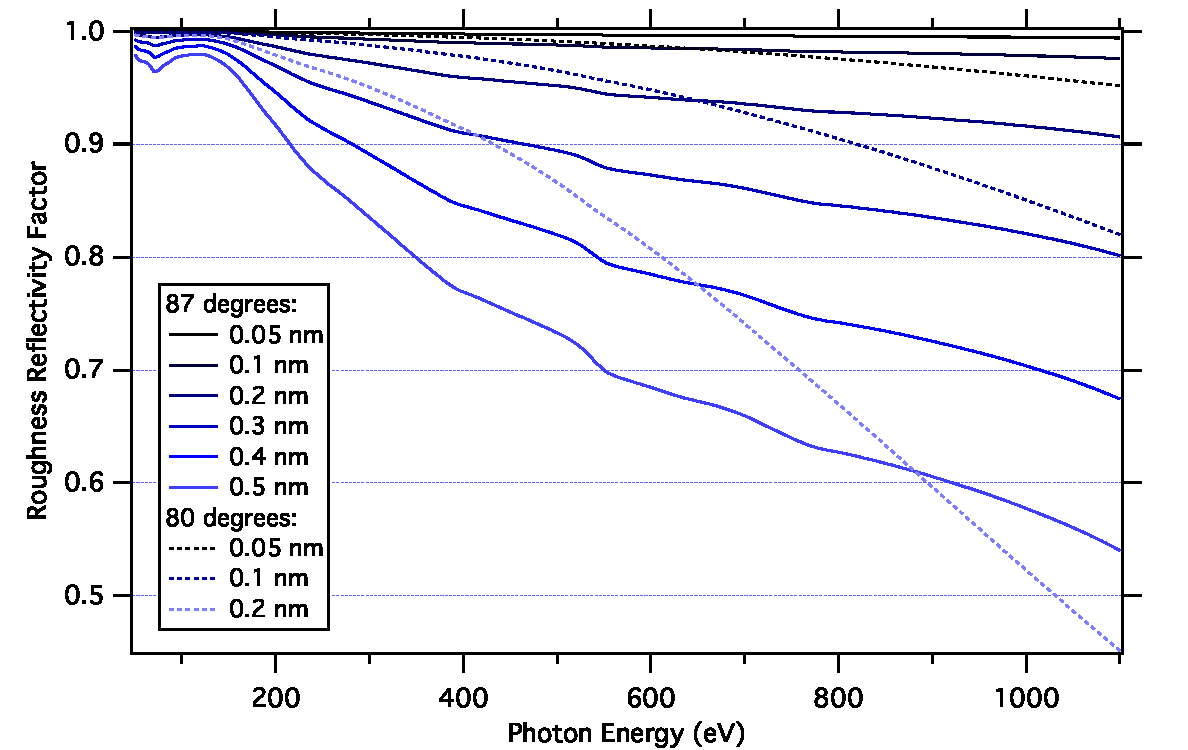
\includegraphics[scale=0.78]{Extended/RoughnessPlots/sinha.pdf} 
   \caption{The reflectivity factor calculated according to the Sinha expression \protect \eq{roughnessCorrection} as a function of incidence angle and photon energy, assuming a refractive index of platinum.}
   \label{sinhaReflectivity}
\end{figure}

\begin{figure}[htbp] %  figure placement: here, top, bottom, or page
   \centering
   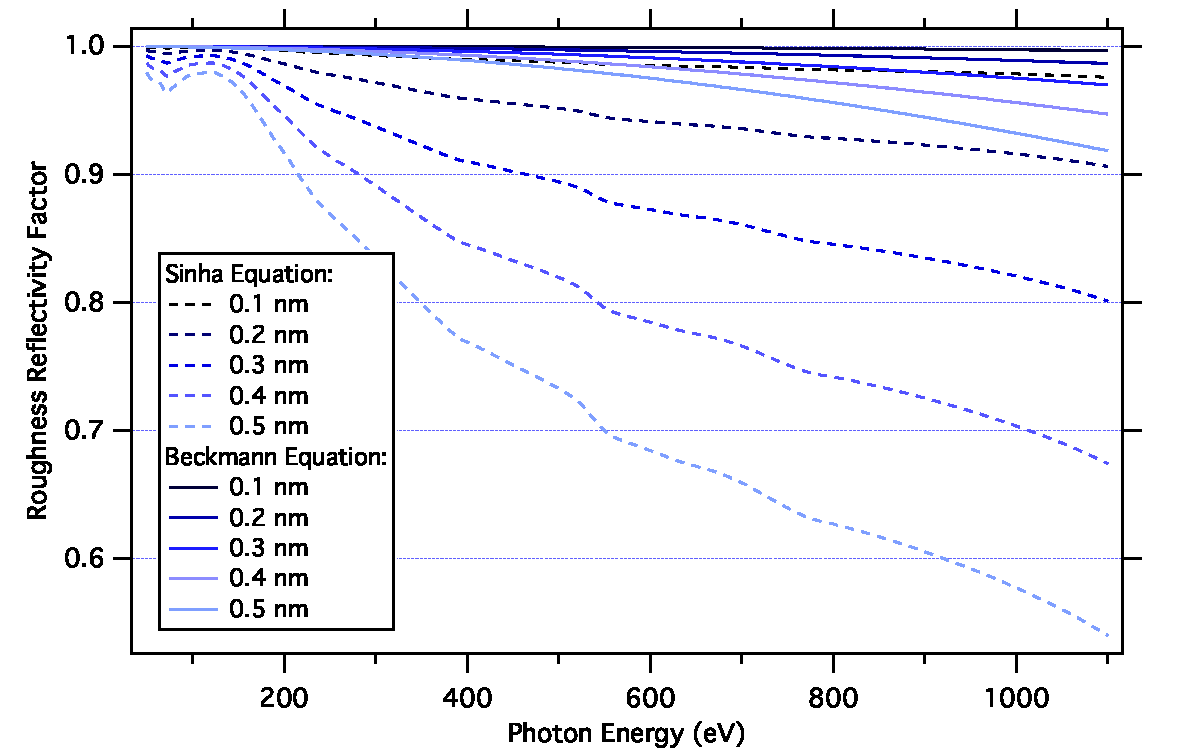
\includegraphics[scale=0.78]{Extended/RoughnessPlots/beckmannAndSinha.pdf} 
   \caption[A comparison of the Beckmann (solid) and Sinha (dashed) expressions for rough surface reflectivity shows the limitations of both approximations.]{A comparison of the Beckmann (solid) and Sinha (dashed) expressions for rough surface reflectivity shows the limitations of both approximations.  (The RMS roughness $\sigma$ is indicated in the legend; the calculations are for 87\dg incidence assuming a refractive index for platinum.)  The Sinha curves incorrectly decrease quickly at high energies (low wavelengths) due to the assumption that $\sigma << \lambda$.  The Beckmann curves show very little reduction even for substantial roughness because the $\cos(\theta)$ term in the Beckmann Equation is only valid near normal, not grazing incidence.}
   \label{beckmannAndSinha}
\end{figure}

If these reflectivity approximations are reasonable, they reinforce how important it is to keep the roughness low during manufacturing.  Our AFM measurements suggest that re-coating the grating after ruling adds to the roughness, due to the granular nature of the evaporated coating.  Due to extensive manufacturing experience, gold coatings are usually the smoothest to apply -- as was the case for our LEG.  The subsequent platinum and nickel over-coatings on the remaining gratings resulted in a much rougher surface.

\subsubsection{Dust, scratches, and pinholes}
Dust, scratches, pinholes, and any other out-of-place bumps on the surface also contribute to the stray radiant energy.  All of these features act as scattering centres and create diffuse light; we can easily confirm this for visible wavelengths (using our biological photodetectors) when looking at a dirty grating under bright light.  Given the challenges of modelling statistically well-behaved surface roughness, we do not even attempt to model these purely random defects, beyond recognizing that they will reduce the overall grating efficiency and contribute to stray light.

\subsubsection{Periodic irregularities of the grooves: ghost peaks}
In the section on grating manufacturing (Section \ref{gratingManufacturing}), we mentioned that periodic errors in the groove position or groove height will create ``ghosts'': additional light intensity peaks superimposed over the desired diffraction pattern.  This happens because the higher-order structure acts like a superimposed grating with its own periodicity.  Just like the other causes of stray radiant energy, if these peaks are present, they will remove energy from the desired diffraction orders, and contaminate the resolution by directing light to the ``right place at the wrong wavelength''.

\subsubsection{Non-periodic irregularities of the grooves}
When ruling a mechanical grating, changes in the elasticity of the metal will allow the tip to penetrate to different depths, causing random (non-periodic) variation in the groove depth from groove to groove.  However, we assumed in Chapter 3 that the grooves were ideally periodic; this assumption is at the core of the differential method.  Therefore, when the shape varies across the grooves, it is impossible to model how this will affect the efficiency.  Further calculations using the integral method -- which does not assume periodicity -- might help answer this question.

If the shape changes slowly across the grating, it might be appropriate to model the overall efficiency as the average of several representative gratings with different shapes.  However, when the shape changes rapidly or randomly, this will reduce the ability of the grating to form regular interfering plane waves, diminishing the diffraction ability.  This has been shown to create a continuous distribution of scattered light which increases as a function of $(1/\lambda^3)$ \cite{Sha78}.

\subsubsection{Irregularities along the groove: out-of-plane reflection}
Another assumption from Chapter 3 was that the grating was invariant along the $z$ direction of the grooves.  The same elasticity changes can cause variation in the shape of the profile as the tip travels along the grooves.  (This also occurs with holographic gratings, due to variation in the mean intensity of the interference pattern during exposure.)  The $z$-variation can reflect light out of the plane of incidence, and the effect can be diffuse or specular \cite{Pal05}.

\subsection{Manufacturing errors that \emph{can} be modelled}
All of the previous real-world grating flaws -- surface roughness, dust and scratches, periodic and non-periodic groove irregularities -- represent deviation from the theoretical profile in Chapter 3 in ways that cannot be incorporated into the model without breaking our initial assumptions (Section \ref{s_assumptions}).  It is also possible for manufacturing errors to create deviation that we \emph{can} actually model; the best example of this would be the difference between the requested and manufactured groove geometry.
\subsubsection{Blaze angle errors shift the efficiency peak}
Figure \ref{3i-2} showed how small changes in the blaze angle can significantly shift the efficiency peak.  For mechanically-ruled gratings, the accuracy of the blaze angle depends on the persistence and perfectionism of the ruling engine operator, who must adjust the diamond tip angle during setup through tedious trial-and-error.  If, after manufacturing, the real blaze angle turns out to be different than what the customer specified, we can measure the true blaze angle using a calibrated AFM and re-calculate the theoretical efficiencies using a better approximation of the profile.

Alternatively, if calibrated AFM measurements are not available, we have determined that the shape of the measured efficiency spectra 
% REALLY?: and the ratio between 1st and 2nd order efficiency
can provide a strong indication of the real blaze angle.  Therefore, we can use a curve-fitting process to choose the best-fit blaze angle that matches the measured to the calculated efficiency curves.  For example, using this technique we predicted a blaze angle of 2.0$\deg$ for the MEG grating, before determining from AFM measurements that the real blaze angle was 2.04$\deg$.  In Section \ref{gratingResults}, we discuss the fitting process and the blaze angle agreement for each grating.

The same technique can be applied to profiles other than blazed gratings; the first method works as long as the groove geometry can be measured.  The second method becomes more time-consuming for profiles like trapezoidal gratings that have more than one adjustable parameter, but this can be accomplished using a multidimensional minimization.

\subsubsection{Deviations from ideal groove shapes affect the efficiency spectrum}
In both mechanically-ruled and holographic gratings, it is likely for the actual groove shape to differ from the ideal rectangular, blazed, and trapezoidal profiles we showed back in Figure \ref{3c-profile}.  If we can determine the actual shape -- for example, from AFM measurements -- we can still model the grating accurately using the differential theory (as long as the profile is still periodic from groove to groove).  Although the \texttt{Gradif} software only supports theoretical shapes, the arbitrary groove profile mode of the new \texttt{PEG} software can be used to model the exact measured shape.  Figure \ref{hegRepresentativeGroove} shows an example of an arbitrary profile extracted from measurements of the HEG.

\subsubsection{Coating oxidation changes the reflectivity}
\label{nickelOxidation}
An unintended consequence of using nickel coated gratings is the unavoidable formation of a thin oxide layer on the surface.  We chose nickel gratings for the IMP and MEG with the intention of using them up to the nickel absorption edge near 850 eV.  However, as is obvious from the NiO reflectivity spectrum in Figure \ref{5f}, we should have expected the oxygen absorption edge to significantly affect their efficiency after 543 eV.  (Besides reducing the overall efficiency, this causes another problem for spectroscopists: when measuring an oxygen emission spectrum using this grating, the efficiency spectrum of the grating oxide will be superimposed on the actual sample measurement.)

While obviously undesirable to have in retrospect, the effect of a surface oxide on the efficiency can be easily modelled using a coating layer on top of a pure metal substrate. In Section \ref{gratingResults} we show how a thin layer of NiO on Ni accounts for the measured efficiency of the IMP and MEG gratings, and we predict the thickness of the oxide layer using fitting.

To protect against the formation of a detrimental oxide, in the future we would request that the grating manufacturer evaporate a layer of MgF$_2$ immediately after applying the primary coating, before exposing the grating to air.  In this case, the effect of the MgF$_2$ layer could also be modelled in the same way.


\begin{figure}[htbp] %  figure placement: here, top, bottom, or page
   \centering
   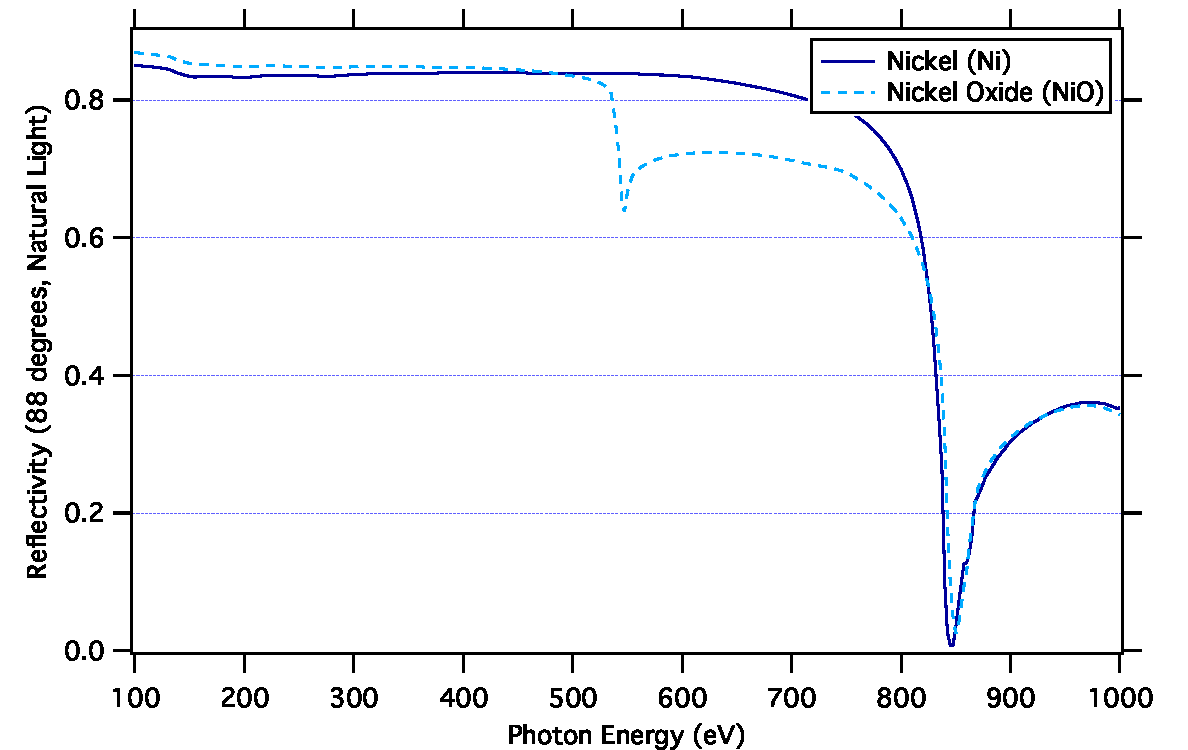
\includegraphics[scale=0.8]{Chapter5/5f_oxidized/Ni_NiO_reflec.pdf} 
   \caption{Unprotected nickel quickly forms a surface oxide of NiO, which significantly reduces the reflectivity at the Oxygen edge (543 eV) }
   \label{5f}
\end{figure}

\section{Grating results, fitting, and comparison to theoretical efficiencies}
\label{gratingResults}
We know that no grating can ever be manufactured exactly as specified, so we would expect the real-world efficiencies to be different than our predictions in Chapter 6.  Is it possible, however, to account for the discrepancies using the differential method?

Given that we have (a) real efficiency measurements over a range of energies, (b) real measurements of the grating geometry, and (c) the ability to model arbitrary groove profiles, we wondered if it would be possible to use a fitting process to generate theoretical efficiency curves that match the measurements, and then compare the fitted parameters to the actual grating parameters.

In this fitting process, we started with fixed values for the parameters that could be measured exactly.  The exact groove densities had been previously determined from power spectral density (PSD) measurements, and confirmed in the diffractometer experiments.  We also took the incidence angles as given, since they were accurately known based on the diffractometer encoders.  Because the blaze angles derived from the AFM measurements showed considerable variation from groove to groove and were subject to uncertainty in the $z$-axis calibration, we left these (and the anti-blaze angles) as free parameters in the fitting process.  The oxide layer thickness for the Ni gratings and the surface roughness parameter $\sigma$ in Equation \eq{roughnessCorrection} were also left as free parameters.
 
 We note that a single efficiency measurement at a single energy would not enable this technique; we need an \emph{efficiency spectrum} measured over a range of energies.  The power of the fitting process comes from the fact that each parameter (groove density, incidence, groove geometry, etc.) affects the \emph{shape} of the spectrum in a different way; the spectral shape acts as a ``fingerprint'' or ``hash'' of the grating parameters.
 
In general, we observed that although the shapes of the measured spectra are similar to the calculated curves, the measurements are always lower than predicted in absolute value.  This is reasonable to expect, according to the number of real-world effects that act to reduce the efficiency: surface roughness, groove variation and irregularities, etc.  Unfortunately, neither the Sinha \eq{roughnessCorrection} nor Beckmann \eq{beckmannFactor} expressions for roughness can describe this well on their own: both of them decrease too rapidly with increasing energy while providing negligible reduction at low energies, and the size of the required parameter $\sigma$ ends up far outside the valid range for the Sinha approximation ($\sigma \ll \lambda$).

Instead, it seems that a \emph{constant scaling factor} is required to achieve a good fit between the measured and calculated spectra.  (Typical scaling values for our measurements are between 0.5 and 0.8.) Although we have described many factors that could account for the reduction, we currently do not have a rigorous physical derivation for this factor.  If it is due to roughness alone, then neither the Beckmann nor Sinha factors are adequate for describing gratings.  It is also possible that this could be a measurement effect; for example, focussing or dispersion of the diffractometer beam by the spherical grating on its way to the photodiode would change the apparent intensity; saggital tilt of the grating would cause some light to miss the photodiode.

Reasonable fitting results can be found by using the same scaling factor for the first-order and second-order efficiencies.  However, much better agreement in the \emph{shapes of the curves} is found using independent scaling factors for the first-order and second-order curves.   Whether this is justifiable depends on the explanation for the scaling factor: both roughness and focussing effects could be affected by the outgoing angle and hence the diffraction order.  We present the results for both methods, and summarize them in Table \ref{fittingResultsTable}.  It turns out that the process using independent scaling factors predicts blaze angles that agree very closely within error of the AFM estimates.  For the nickel coated gratings, it also predicts lower oxide thicknesses than using a common scaling factor.

\subsection{Low Energy Grating (LEG)}
%  (gold): profile clean; as expected; blaze angle off. [modelled]
The LEG was one of the easiest gratings to manufacture, due to its low groove density and lack of a secondary coating.  It was ruled directly into a layer of gold on the surface of the substrate, and the AFM measurements (Figure \ref{5y-leg}) show a clean triangular profile at the centre of the grating.  However, the estimated actual blaze angle based on AFM measurements at the centre of the grating is $2.45\deg \pm 0.20\deg$, a substantial difference from the nominal 1.85\dg we specified.

\begin{figure}[htbp] %  figure placement: here, top, bottom, or page
   \centering
   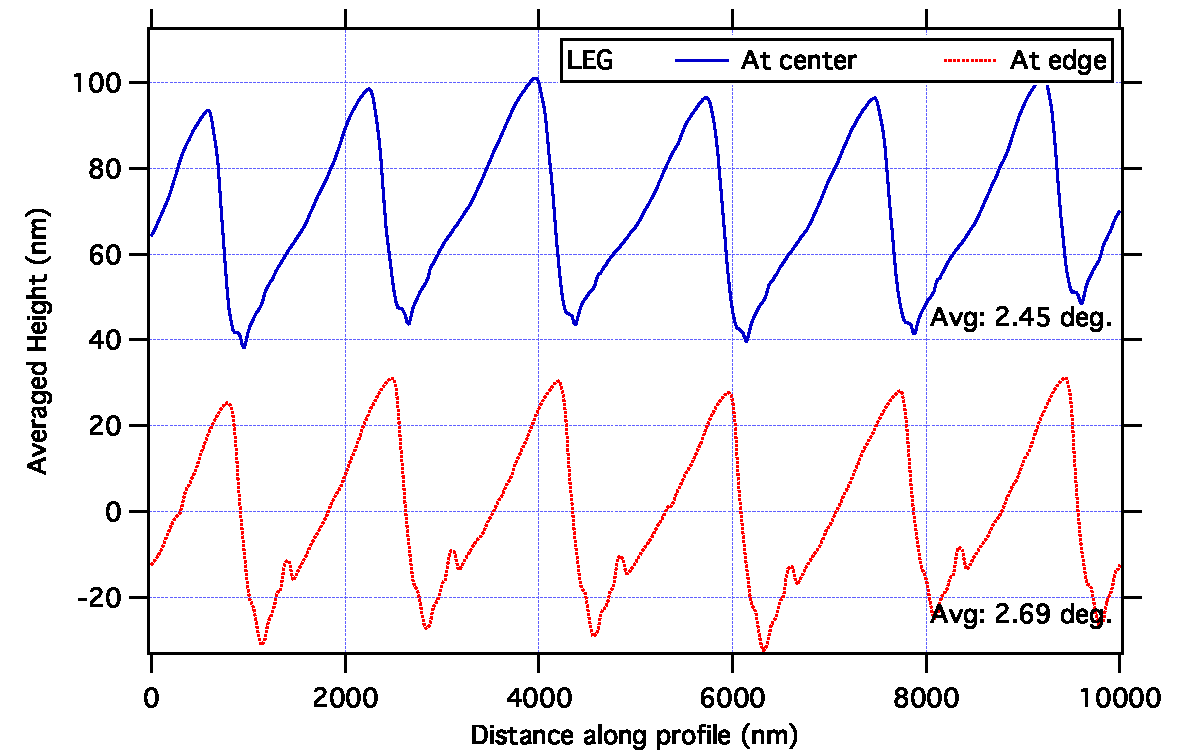
\includegraphics[scale=0.7]{Chapter5/5y_afm/LEG.pdf} 
   \caption{AFM measurements of the Low Energy Grating (LEG) profile, averaged along the grooves (10 um $\times$ 10 um).  The best-fit blaze angle at the centre of the grating is $2.45\deg \pm 0.20\deg$.}
   \label{5y-leg}
\end{figure}
The effect of the blaze angle error on the measured efficiency is obvious in Figure \ref{5x-leg}: the locations of the efficiency peaks are shifted compared to the theoretical prediction for a nominal grating with 1.85$^\circ$ blazing.  A higher blaze angle also increases the second-order peak efficiency at the expense of the first.

When we use a fitting process to match the theoretical curves to the measured efficiency, it predicts a blaze angle of $2.35\deg$, using scaling factors of 0.93 and 0.84 for the first and second orders respectively.   The agreement in the shape of the curves is very good (Figure \ref{5x-leg}), and the predicted blaze angle agrees closely with the AFM estimate ($2.45\deg$).  The high scaling factors compared to the IMP and MEG gratings suggests a high smoothness; it makes sense that the over-coated gratings would be rougher than the bare gold.

If we insist on a common scaling factor for both first and second order, the fitting process predicts a blaze angle of 2.26\dg and a scaling factor of 0.95.  We can see in Figure \ref{LEGSingleScaling} that this reduces the agreement between the measured and fitted curves; it also provides a less accurate prediction of the blaze angle.

Although only a fraction of a degree, the blaze angle error causes a significant reduction in real-world efficiency.  At 140 eV, the theoretical and measured efficiency is less than 0.3, compared to the 0.4 that it could have been with correct blazing.  Fortunately, this is still high compared to the other gratings and should be acceptable for all experiments.

\begin{figure}[htbp] %  figure placement: here, top, bottom, or page
   \centering
   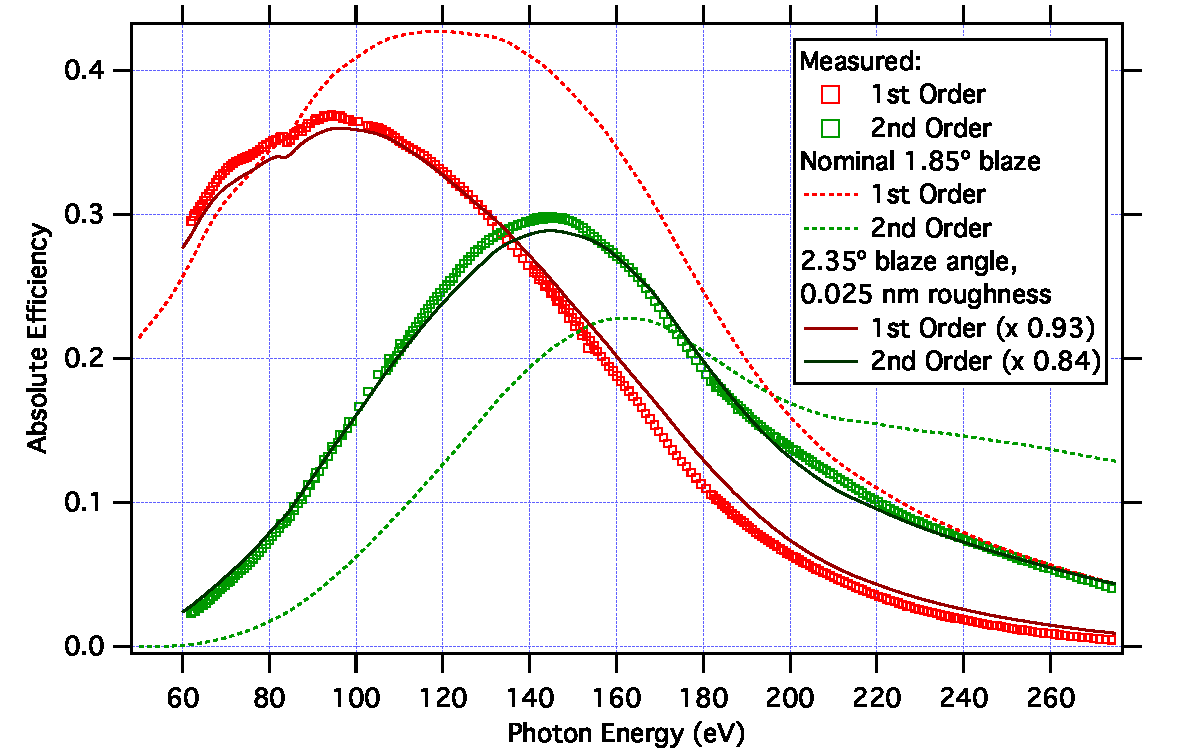
\includegraphics[scale=0.7]{Extended/legFitting/LEGFittedDoubleScaling.pdf} 
   \caption{The blaze angle error of the manufactured LEG causes the efficiency peak to shift down in energy, and causes a transfer of energy from the first order to the second order.  The fitting process predicts a blaze angle of $2.35\deg$ and an RMS roughness of 0.025 nm.  (This assumes scaling factors of 0.93 and 0.84 for the first and second order respectively.)  The predicted blaze angle agrees within error with the AFM estimate ($2.45\deg$).}
   \label{5x-leg}
\end{figure}

\begin{figure}[htbp] %  figure placement: here, top, bottom, or page
   \centering
   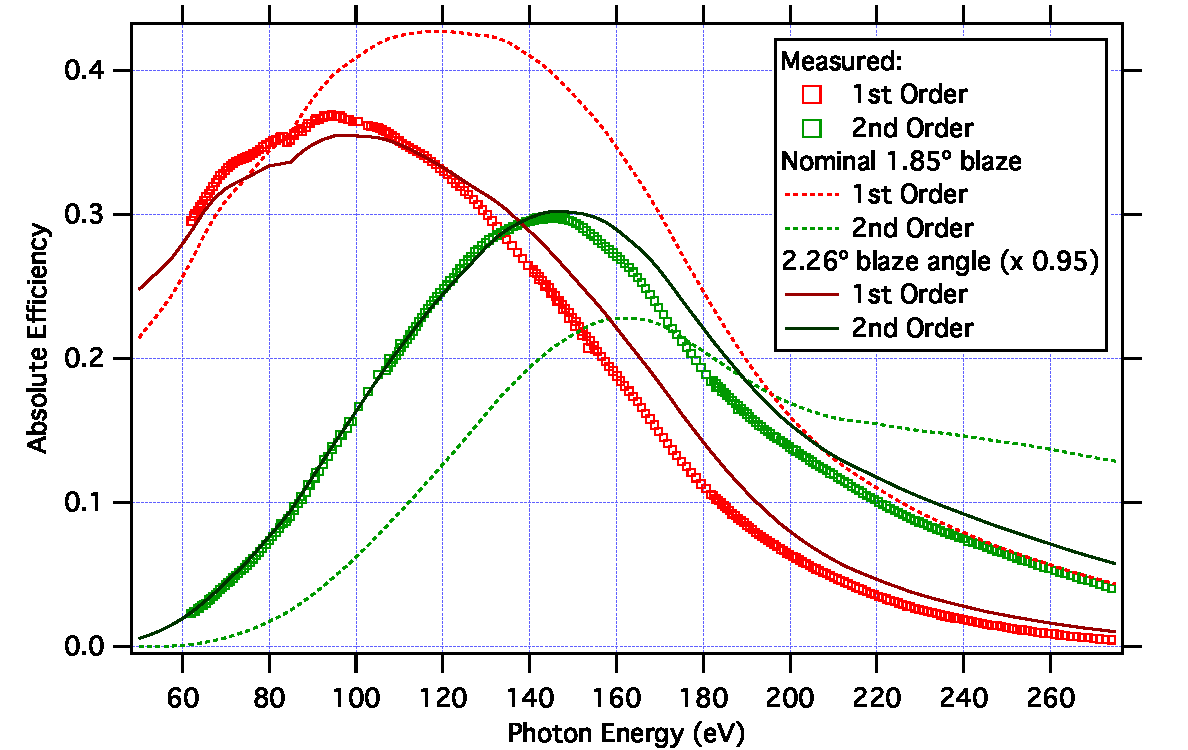
\includegraphics[scale=0.7]{Extended/legFitting/LEGFittedSingleScaling.pdf} 
   \caption{When using a common scaling factor for fitting the LEG, we predict a blaze angle of $2.26\deg$ and a scaling factor of 0.95.  However, this method provides less agreement and a less accurate blaze prediction than using independent scaling factors (Figure \ref{5x-leg}).}
   \label{LEGSingleScaling}
\end{figure}

\subsection{Impurity Grating (IMP)}
The AFM measurements of the impurity grating show clean facets on the blazed side (Figure \ref{5y-imp}), although once again the blaze angle is higher than specified: the best-fit angle at the grating centre is $1.60\deg \pm 0.11\deg$, compared to the nominal 1.11$^\circ$.  This is consistent with the LEG, which also overshot the nominal blaze angle by $0.4\deg - 0.5\deg$.

\begin{figure}[htbp] %  figure placement: here, top, bottom, or page
   \centering
   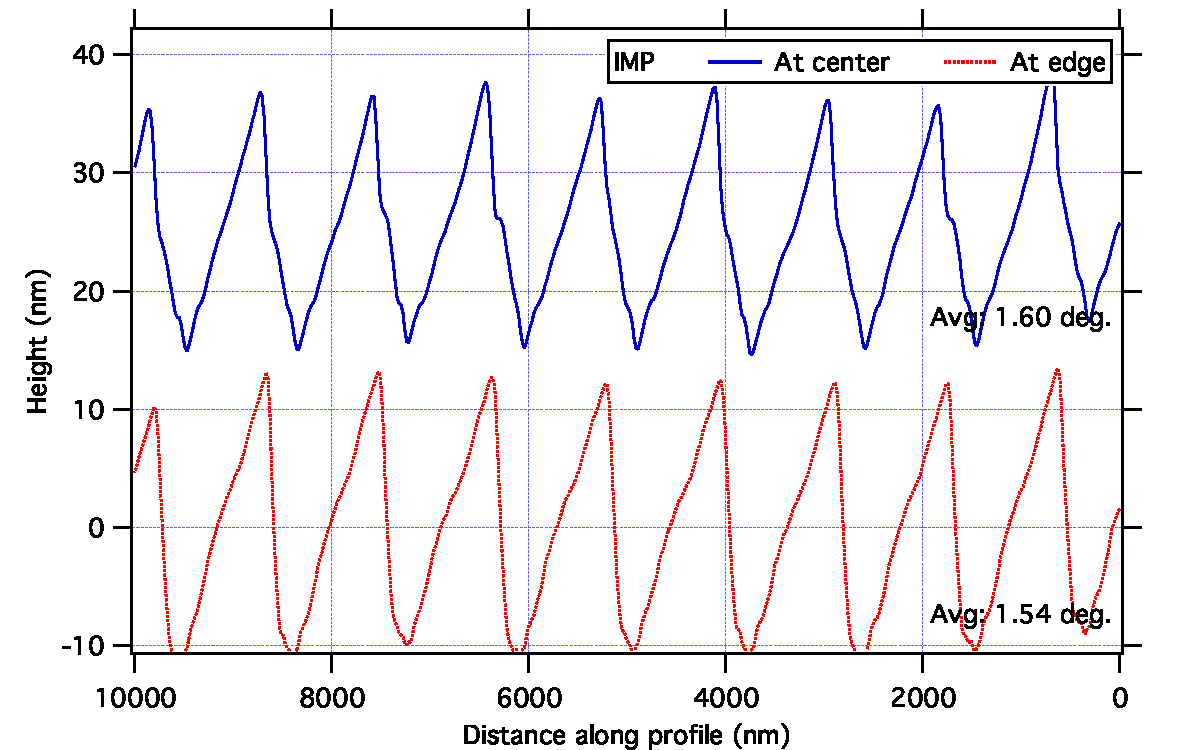
\includegraphics[scale=0.7]{Chapter5/5y_afm/IMP.pdf} 
   \caption{AFM measurements of the Impurity Grating (IMP) profile, averaged along the grooves (10 um $\times$ 10 um).  The best-fit blaze angle at the centre of the grating is $1.60\deg \pm 0.11\deg$.}
   \label{5y-imp}
\end{figure}

Originally intended to cover the range from 200 to 800 eV, the IMP suffers a noticeable drop in measured efficiency near 540 eV (Figure \ref{5x-imp}).  It is easy to recognize that this occurs at the onset of the oxygen absorption edge (543 eV), suggesting an oxide layer on the surface.  Fitting using a common scaling factor for first and second order predicts a blaze angle of $1.4\deg$, a scaling factor of 0.9, and a 7 nm coating of NiO on top of the Ni surface (Figure \ref{singleScalingFit}).  However, the best fit to the shape of the curves comes from using separate scaling factors, and suggests that the measured spectrum can be explained by a blaze angle of $1.65\deg$, a $5\deg$ anti-blaze angle, a 2.0 nm oxide layer, an RMS roughness of 0.5 nm, and scaling factors of 0.91 and 0.62 respectively (Figure \ref{5x-imp}).  We have not found a way to confirm the oxide and roughness predictions, but the blaze angle predicted from fitting agrees closely within error of the AFM estimate ($1.60\deg$).

Another interesting observation is that we should not expect the Henke data to be accurate near the oxygen and nickel edges; however, the calculated efficiencies actually reproduce the fine structure visible in the measurements from 540 to 560 eV.

\begin{figure}[htbp] %  figure placement: here, top, bottom, or page
   \centering
   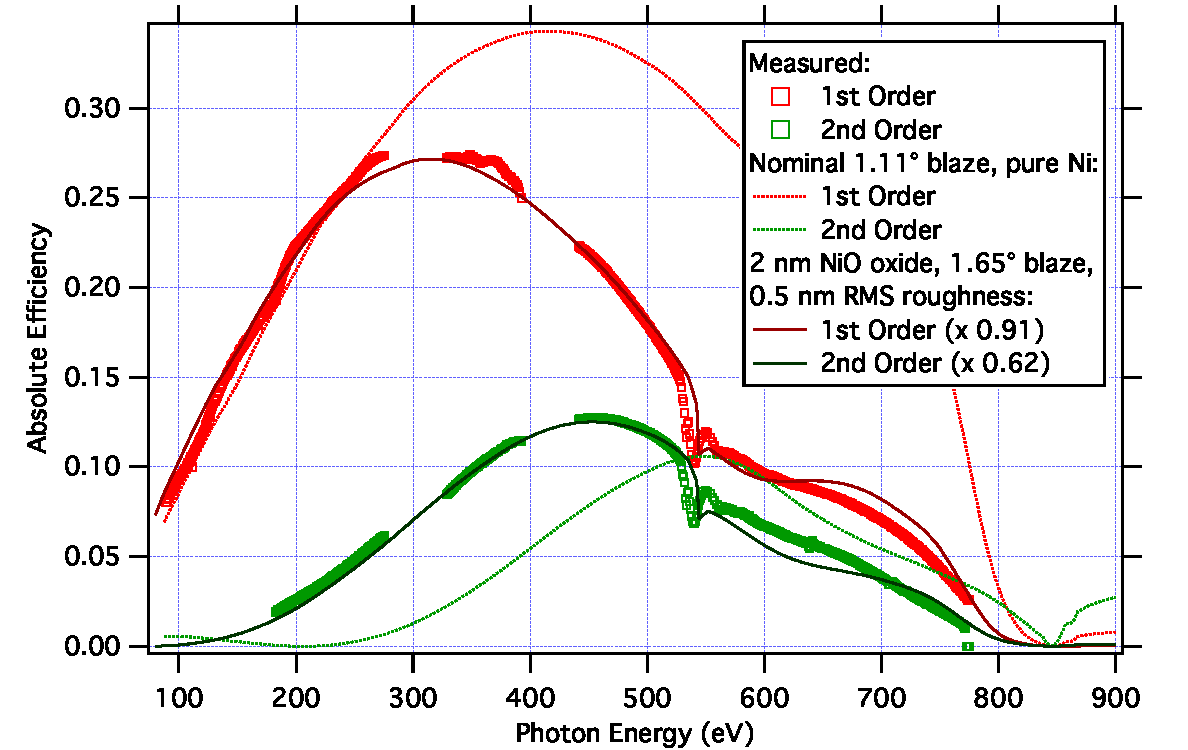
\includegraphics[scale=0.7]{Extended/impFitting/IMPFittedDualScaling.pdf} 
   \caption{Theoretical and measured efficiency of the Impurity Grating (IMP).  The best-fit theoretical curve predicts a blaze angle of $1.65\deg$, an anti-blaze angle of $5\deg$, a 2.0 nm oxide layer, and an RMS roughness of 0.5 nm.  (This assumes that the first order calculated efficiency is scaled by 0.91, and the second order is scaled by 0.62.)  The fitting prediction agrees closely with the AFM estimate of the blaze angle ($1.60\deg$).}
   \label{5x-imp}
\end{figure}

\begin{figure}[htbp] %  figure placement: here, top, bottom, or page
   \centering
   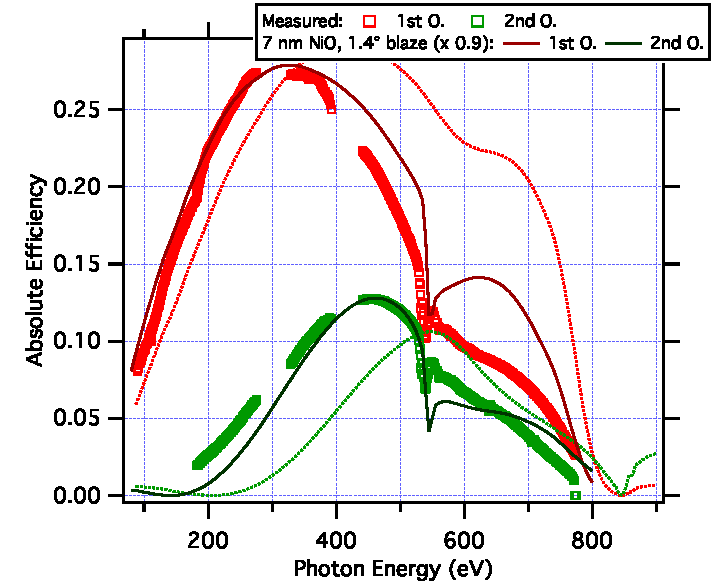
\includegraphics[width=0.49\textwidth]{Extended/impFitting/IMPFittedSingleScaling_small.pdf} 
     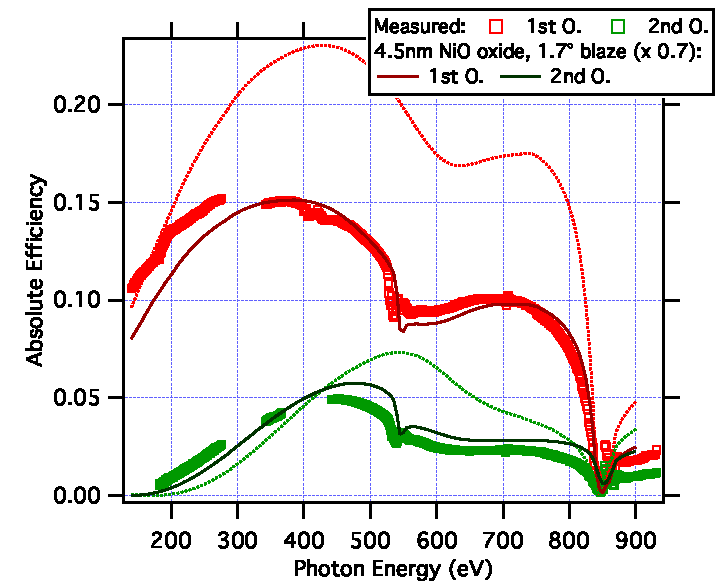
\includegraphics[width=0.49\textwidth]{Extended/megFitting/MEGFittedSingleScaling_small.pdf} 
   \caption{Using a common scaling factor for the first-order and second-order efficiency curves reduces the fitting accuracy and reduces the agreement between the predicted and AFM estimated blaze angles.  For the impurity grating (left), this process predicts a $1.40\deg$ blaze angle, a 7 nm NiO surface layer, and a scaling factor of 0.9.  For the MEG (right), it predicts a $1.7\deg$ blaze angle, a 4.5 nm NiO layer, and a scaling factor of 0.7.}
   \label{singleScalingFit}
\end{figure}

\subsection{Medium Energy Grating (MEG)}
The MEG, with an increased groove density of 1200 lines/mm, shows a less regular surface than either the LEG or IMP.  AFM measurements of the profile (Figure \ref{5y-meg}) estimate an average blaze angle of $2.04\deg \pm 0.22\deg$ at the centre of the grating.  Again, this is consistently $0.5\deg$ higher than the nominal specification of $1.48\deg$.

\begin{figure}[htbp] %  figure placement: here, top, bottom, or page
   \centering
   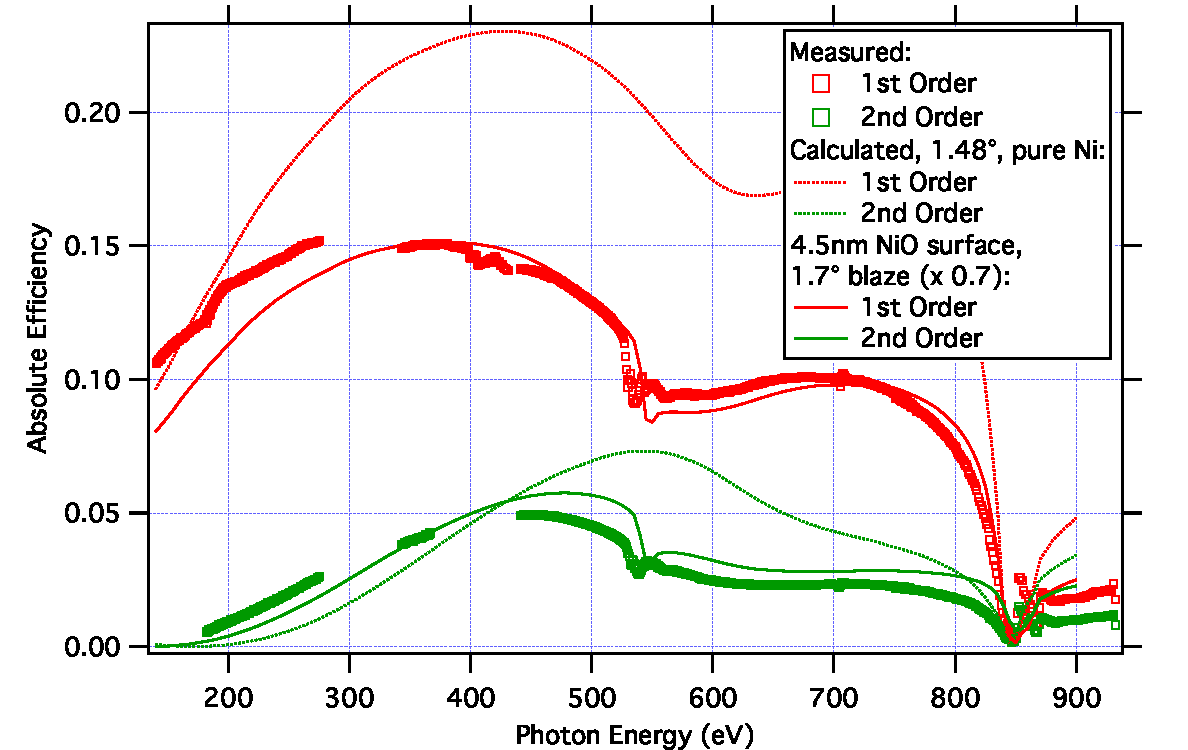
\includegraphics[scale=0.7]{Chapter5/5y_afm/MEG.pdf} 
   \caption{AFM measurements of the Medium Energy Grating (MEG) profile, averaged along the grooves (5 um $\times$ 5 um).  The best-fit blaze angle at the centre of the grating is $2.04\deg \pm 0.22\deg$.}
   \label{5y-meg}
\end{figure}

In efficiency, the nickel MEG suffers the same fate as its oxidized sibling.  The measured efficiency (Figure \ref{5x-meg}) is further affected by the error in the blaze angle.  The best-fit calculations predict a blaze angle of $1.95\deg$, an NiO oxide layer of 1 nm, and scaling factors of 0.70 (first order) and 0.37 (second order).  The lower scaling factors are attributed to the significant groove variation visible in the AFM profile compared to the smoother LEG and IMP.  Again, the fitted blaze angle agrees closely with the AFM estimate ($2.04\deg$).  A worse fit is obtained using a single scaling factor of 0.7, giving a $1.7\deg$ blaze angle and 4.5 nm oxide layer.

\begin{figure}[htbp] %  figure placement: here, top, bottom, or page
   \centering
   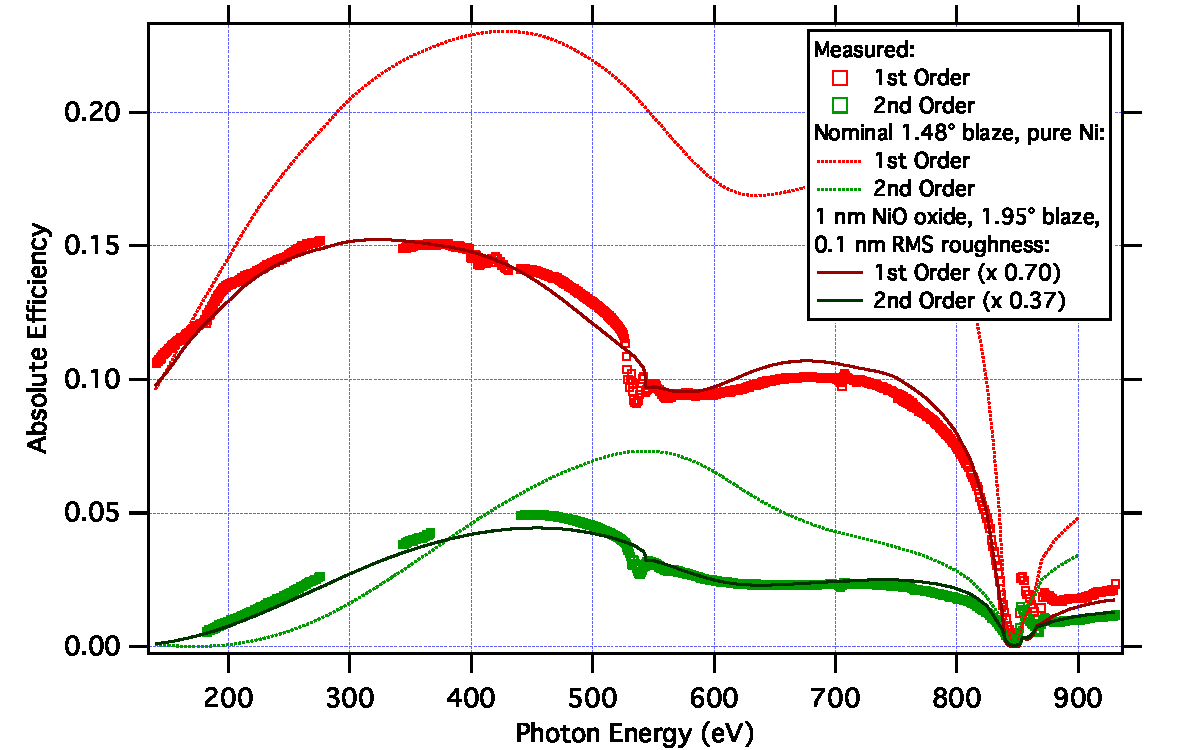
\includegraphics[scale=0.7]{Extended/megFitting/MEGFittedDoubleScaling.pdf} 
   \caption{The real-world efficiency of the MEG can be explained by the fitting process, which predicts a blaze angle of $1.95\deg$, an anti-blaze angle of $30 \deg$, a 1 nm coating of nickel oxide (NiO), and a surface roughness of 0.1 nm RMS.  The scaling factors for first and second order are 0.70 and 0.37 respectively. }
   \label{5x-meg}
\end{figure}

\subsection{High Energy Grating (HEG)}
When we measured the diffraction efficiency of the HEG grating, we were surprised to observe almost no diffraction in the first and second order (Figure \ref{5x-heg}); initially we thought we had mistakenly mounted it backwards in the diffractometer.  On closer inspection, the diffraction peaks were found, but the measured efficiency spectrum is unusably low across the whole energy range.

\begin{figure}[htbp] %  figure placement: here, top, bottom, or page
   \centering
   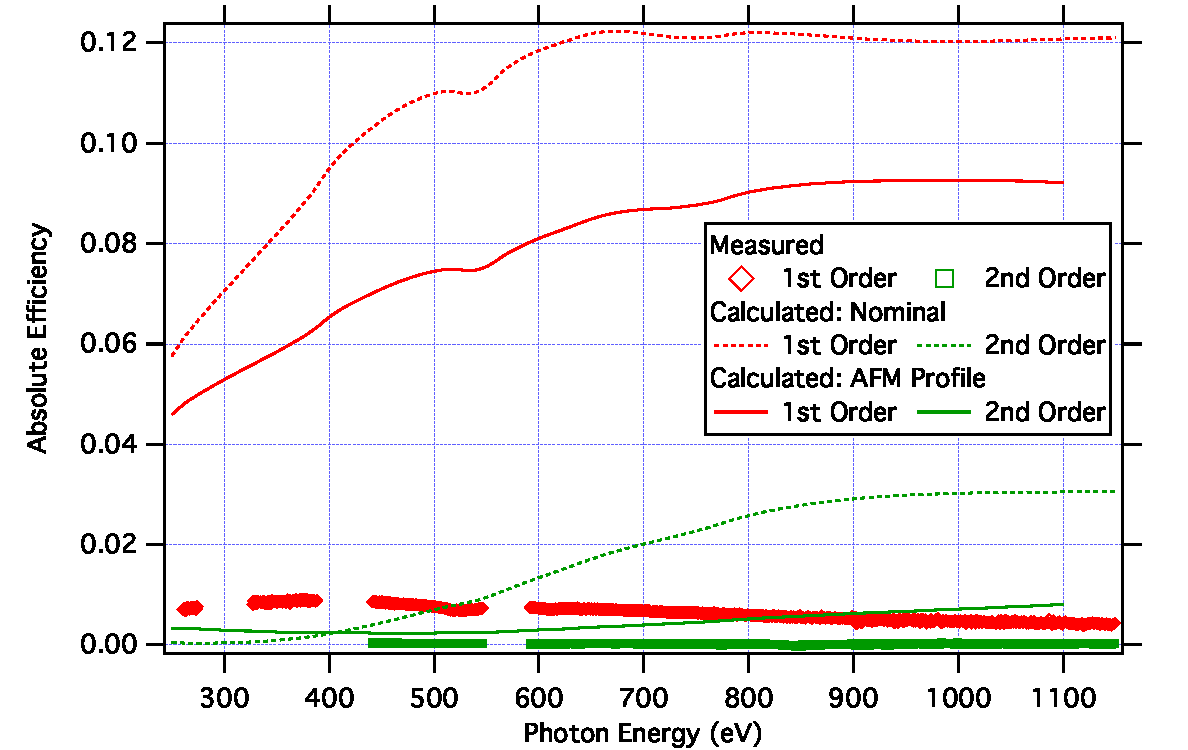
\includegraphics[scale=0.7]{Extended/HEGCustomProfile/HEG_2.pdf} 
   \caption{Theoretical and measured efficiency of the High Energy Grating (LEG).  The solid theoretical curves were calculated using an arbitrary groove shape based on the AFM measurements (Figure \ref{hegRepresentativeGroove}).  It cannot fully explain the reduction in real-world efficiency; therefore, we attribute the poor performance to groove-to-groove variation and scatter that we cannot model using the differential method.}
   \label{5x-heg}
\end{figure}

What could have caused this? It is easy to see from the AFM measurements of the HEG (Figure \ref{5y-heg}) that something went very wrong in the ruling process.  At the centre of the grating, there is a double-peaked structure, and the dimensions differ substantially from groove to groove.  We know that the HEG blank was re-ruled after a previous failed attempt by the manufacturer, and we can hypothesize that some structure was left over from the first ruling.

\begin{figure}[htbp] %  figure placement: here, top, bottom, or page
   \centering
   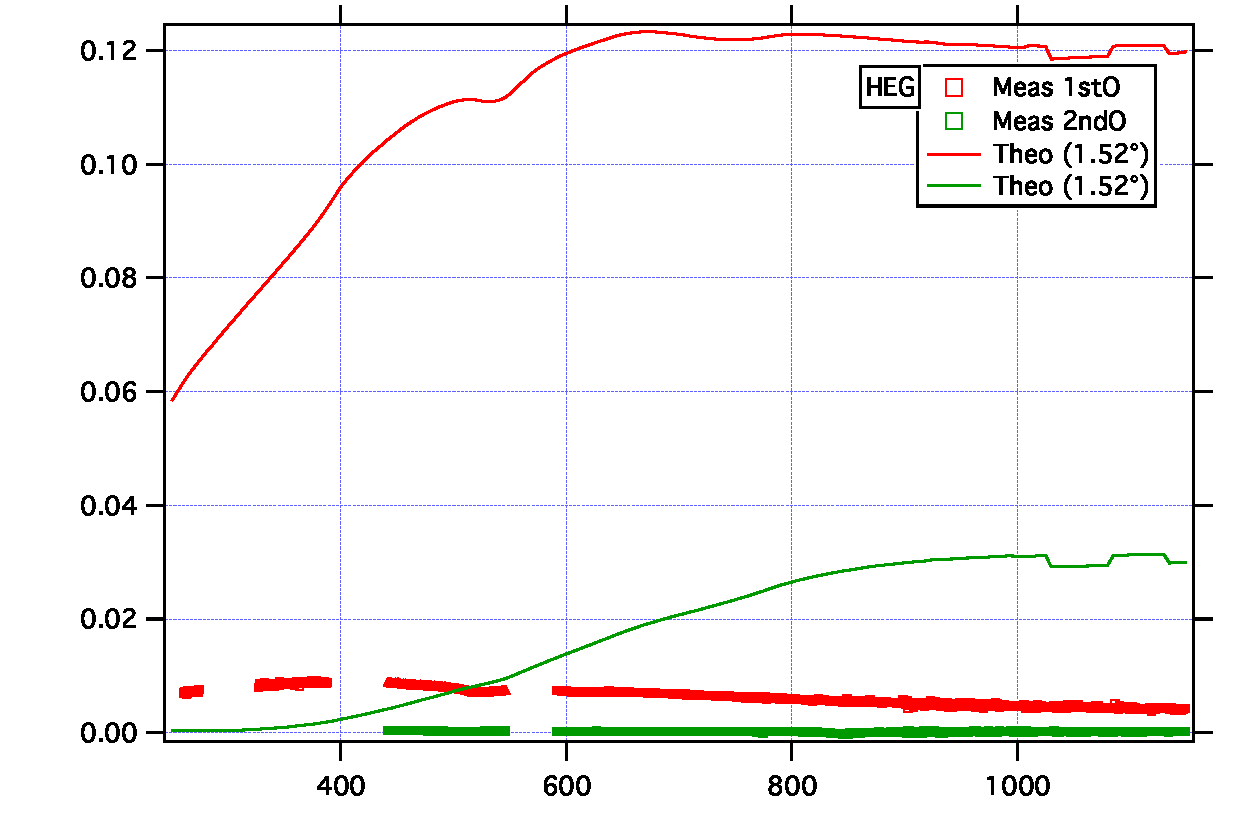
\includegraphics[scale=0.7]{Chapter5/5y_afm/HEG.pdf} 
   \caption{AFM measurements of the High Energy Grating (HEG) profile, averaged along the grooves (5 um x 5 um).  Severe ruling errors were apparent.  The profile wasn't sufficiently triangular to attempt to fit a blaze angle, so we extracted one of the groove shapes to model as an arbitrary profile (Figure \ref{hegRepresentativeGroove}).}
   \label{5y-heg}
\end{figure}

\begin{figure}[htbp] %  figure placement: here, top, bottom, or page
   \centering
   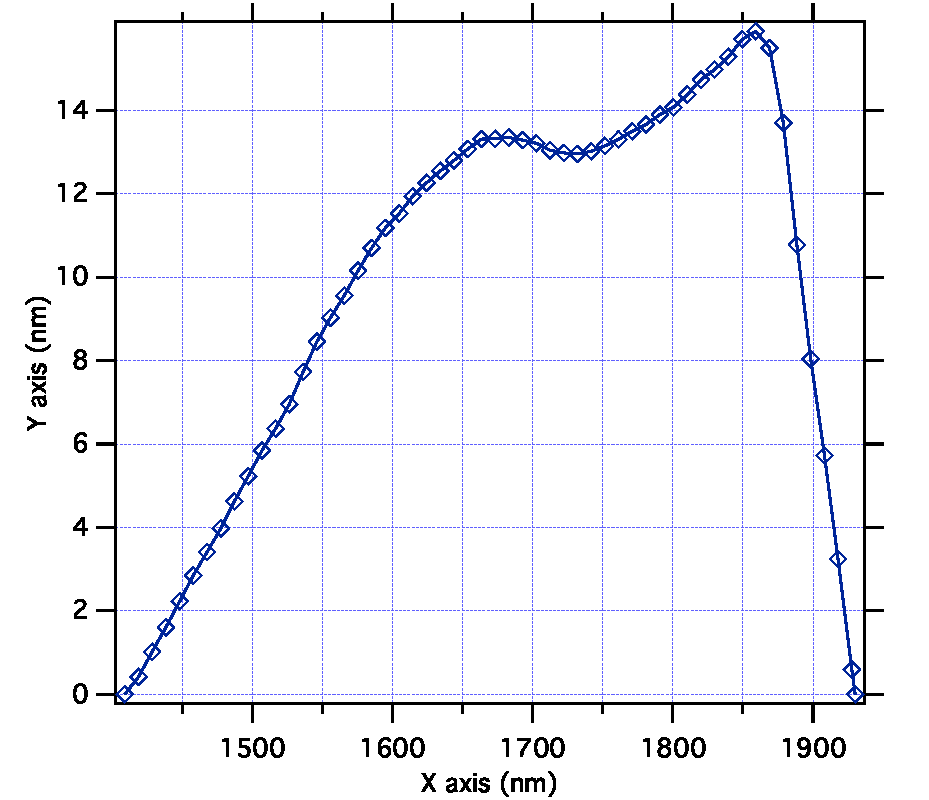
\includegraphics[scale=0.7]{Extended/HEGCustomProfile/representativeProfile.pdf} 
   \caption{Representative profile used to model the real-world HEG, extracted from the AFM measurements in Figure \ref{5y-heg}.}
   \label{hegRepresentativeGroove}
\end{figure}

This grating highlights the importance of careful characterization.  In this form, the HEG would have been unusable.

Without efficiency and AFM measurements, we would have accepted and installed this grating in the spectrometer, only to be perplexed at the inability to detect anything other than scattered light.   Instead, we were able to use this data to persuade the manufacturer to re-rule it one more time.\footnote{Coincidently or un-coincidently, the manufacturer also purchased their own AFM after this exchange.  Currently we are still waiting for delivery of the final grating.}

Could the double-peaked shape of the HEG grooves be responsible for the poor efficiency?  This question provided an opportunity to test out the arbitrary profile mode of the new \texttt{PEG} software.  We extracted a representative shape from one of the AFM grooves (plotted in Figure \ref{hegRepresentativeGroove}) and used it to specify the set of $(x,y_p)$ points for the profile function $y_p = g(x)$.

The efficiencies calculated using this groove shape are also shown in Figure \ref{5x-heg}.  While the double-peaked shape does indeed reduce the theoretical efficiency compared to the nominal profile, it cannot explain the near-zero efficiencies that we measured.  Instead, we attribute this to the strong non-periodic variation from groove to groove, which disrupts the formation of diffracting plane waves.  (In the limit of complete random variation from groove to groove, the grating simply becomes a rough diffuse surface, scattering in all directions.)

% Requires the booktabs if the memoir class is not being used
\begin{table}[htbp]
   \centering
   \topcaption[Comparison of actual and predicted grating parameters, using fitting to match the calculated efficiency spectra to the measured curves.]{Comparison of actual and predicted grating parameters, using fitting to match the calculated efficiency spectra to the measured curves.  The fitting process was done using a common scaling factor (CF) and independent scaling factors (IF) for the first- and second-order curves, and Equation \protect \eq{roughnessCorrection} for the surface roughness correction.  Using independent scaling factors provides the best agreement with the measurements and very accurate blaze angles compared to the AFM estimates.} % requires the topcapt package
   \begin{tabular}{@{} llllllll @{}} % Column formatting, @{} suppresses leading/trailing space
      \toprule
    &  \multicolumn{3}{l}{Blaze Angle ($\deg$)} & \multicolumn{2}{l}{Roughness (nm RMS)} &  \multicolumn{2}{l}{Oxide Thickness (nm)} \\
      \cmidrule(lr){2-4}    \cmidrule(lr){5-6}    \cmidrule(lr){7-8}  
 &	Fit (CF) & Fit (IF) & AFM Estimate & Fit (CF) & Fit (IF) &  Fit (CF) & Fit (IF)\\
 \cmidrule(lr){2-2}   \cmidrule(lr){3-3} \cmidrule(lr){4-4} \cmidrule(lr){5-5} \cmidrule(lr){6-6}  \cmidrule(lr){7-7}  \cmidrule(lr){8-8}
LEG & 2.26 & 2.35 & 2.45 $\pm$ 0.20 & -- & 0.025 & N/A & N/A \\
IMP & 1.40 & 1.65 & 1.60 $\pm$ 0.11 & -- & 0.5 & 7.0 & 2.0 \\
MEG & 1.70 & 1.95 & 2.04  $\pm$ 0.22 & -- & 0.1 & 4.5 & 1.0\\
      \bottomrule
   \end{tabular}
   \label{fittingResultsTable}
\end{table}

\subsection{High resolution third-order gratings}
The high-resolution third-order gratings (HRMEG and HRHEG) were also characterized using AFM and diffractometer measurements.  Unfortunately, the diffractometer measurements were affected by an issue in the diffractometer control software that caused errors in the normalization.  It might be possible to correct this problem with post-processing, but at the moment the full efficiency spectra are not ready for publication.  We include summary results from the valid measurement points here.

\subsubsection{HRMEG}
The nickel-coated HRMEG has a measured third-order efficiency peak of 3.5\%, but unfortunately the peak occurs at 500 eV instead of the 285 eV design energy.  Like the other two nickel gratings, it shows fine structure and a serious decrease in efficiency at the oxygen edge (543 eV).  AFM measurements of the HRMEG profile show a beautiful triangular structure (Figure \ref{5y-hrmeg}); unfortunately the best-fit blaze angle is $4.43\deg \pm 0.30\deg$ at the centre of the grating.  Unlike the other gratings, this is $0.4\deg$ \emph{lower} than the nominal $4.85\deg$ we requested.  Again, the blaze angle error explains why the measured efficiency peak is shifted compared to the nominal calculations, although in this case it shifts to higher instead of lower energies.  The effect on the spectrometer performance is nearly a factor of two: instead of the $>3\%$ third-order efficiency we could get at 285 eV with the proper blaze, we see only 1.5\%.

\begin{figure}[htbp] %  figure placement: here, top, bottom, or page
   \centering
   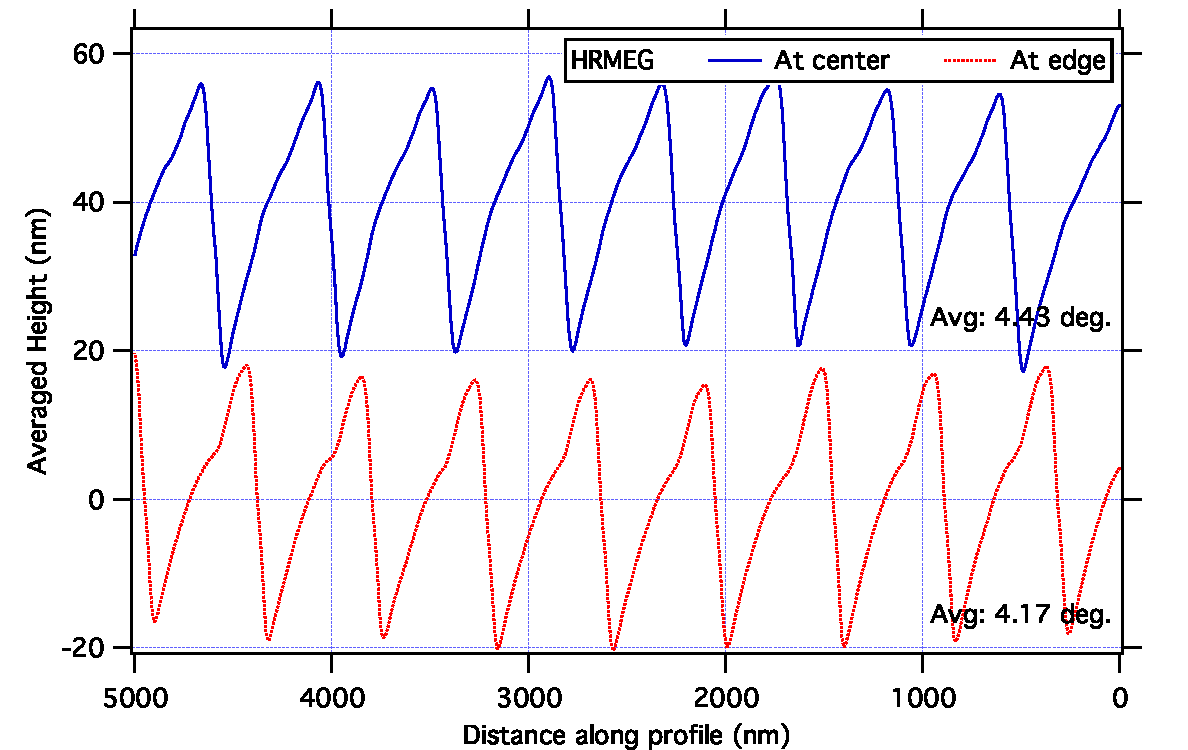
\includegraphics[scale=0.7]{Chapter5/5y_afm/HRMEG.pdf} 
   \caption{AFM measurements of the HighRes Medium Energy Grating (HRMEG) profile, averaged along the grooves (5 um x 5 um).  The best-fit blaze angle at the centre of the grating is $4.43\deg \pm 0.30\deg$.}
   \label{5y-hrmeg}
\end{figure}

\subsubsection{HRHEG}
The HRHEG was the most challenging grating to rule due to its extremely high groove density of 2600 lines/mm.  As a result, we should not expect a very smooth profile.  However, AFM measurements show that this grating is exceptionally far from meeting the blaze angle specification.  Figure \ref{5y-hrheg} reveals an extremely high blaze angle of $6.34 \pm 0.28\deg$ -- more than two degrees higher than the required $4.05\deg$.  Since accurate blazing is essential for exploiting the third-order efficiency peak, it was unfeasible to use this grating in the role we originally designed it for: the third-order efficiency is less than 0.5\% at 400 eV, and decreases to 0.28\% at the design energy of 725 eV.

However, this blaze angle error had an unintended but lucky consequence: it actually makes the HRHEG ideally blazed for \emph{first order} operation from 400 eV to 900 eV.  (Although the efficiencies are low due to the extreme groove density, it was measured to give 2\% efficiency at 400 eV, and $>1\%$ efficiency at 800 eV.)  Simultaneously, the failure of the \emph{HEG} left us lacking a general first-order grating to support experiments above 530 eV.  Therefore, we had the idea to install the HRHEG in the spectrometer as a temporary first-order HEG replacement until the manufacturer was done re-ruling the actual HEG.  Fortunately, the manufacturer also had a spare blank (substrate) for the HRHEG, so they could proceed with ruling another copy of it as well.  This example again highlights the value of careful characterization from an engineering perspective.

\begin{figure}[htbp] %  figure placement: here, top, bottom, or page
   \centering
   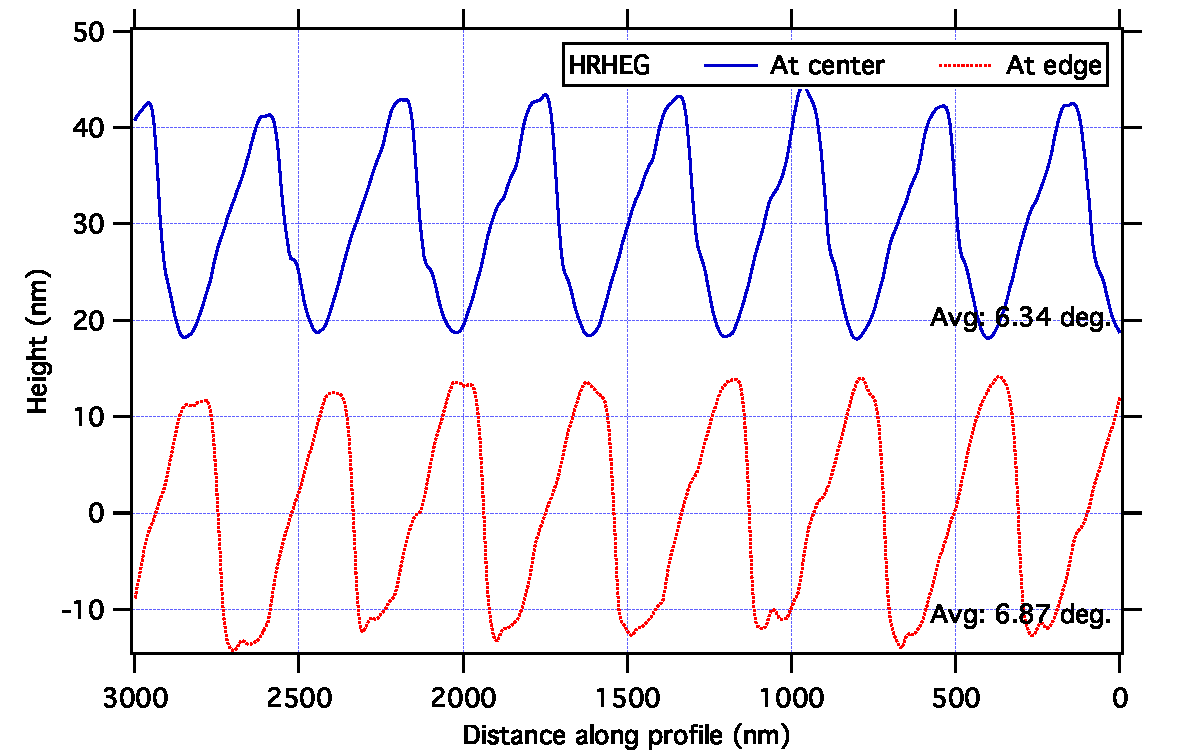
\includegraphics[scale=0.7]{Chapter5/5y_afm/HRHEG.pdf} 
   \caption{AFM measurements of the HighRes High Energy Grating (HRHEG) profile, averaged along the grooves (3 um x 3 um).  The best-fit blaze angle at the centre of the grating is $6.34\deg \pm 0.28\deg$.}
   \label{5y-hrheg}
\end{figure}
